% !TEX root = ./master.tex
\chapter[\'Etude clinique]{\'Etude clinique}

%Souvenons-nous brièvement de l'évolution de la signification du terme
%``clinique'' enraciné dès l'Antiquité.
%A l’origine,\textbf{ l’activité clinique} (<gr. klinê = le lit) est celle du médecin qui, au chevet du malade, procède à l’examen des manifestations de la maladie (méthode de l’observation, de l’interrogation et de l’écoute) en vue de poser un diagnostic*, un pronostic* et une prescription* de traitement.
%Michel Foucault (1926-†1984), psychologue français, dans son ouvrage capital de 1963,
%«Naissance de la clinique» nous rend attentifs au fait que l’adjectif «clinique» fut longtemps du monopole médical, avec %l’observation « naturelle » faite au lit du malade, uniquement à l’aide des organes sensoriels.

%Hippocrate (médecin grec, Cos 460-377) était clinicien : il apprenait à ses étudiants l’art d’observer les symptômes, ceux-ci étant les réactions d’une personnalité à une agression pathogène. Généralisation et rationalisation, selon les critères d’Aristote, permettaient l’élaboration de « ces entités nosologiques* », les maladies, qui s’emparaient du corps du malade et poussant les médecins, exorcistes laïques, à les en faire sortir.
%Les publications de Th.Ribot à la Sorbonne rejoignent [avec «La psychologie des sentiments »(1896), «Les maladies de la mémoire »(1883) et «Les maladies de la personnalité » (1885)], les idées de S. Freud, montrant la primauté de la vie affective, où les tendances inconscientes jouent un rôle fondamental, et pouvant s’extérioriser soit par l’arrêt du développement affectif, soit par la dissolution des acquisitions plus récentes.

%L’expression « psychologie clinique » apparaît sous la plume de S. Freud, dans sa lettre à W. Fliess du 30.01.1899 : « Maintenant, la connexion avec la psychologie, telle qu’elle se présente sur les Etudes sur l’hystérie(1895) sort du chaos, j’aperçois les relations avec le conflit, la vie, tout ce que j’aimerais appeler psychologie clinique ».

%La définition « officielle » de la psychologie clinique mobilise et articule la singularité et
%la totalité, de façon à reconnaître une discipline psychologique basée sur l’étude approfondie des cas individuels, l’étude de la conduite humaine individuelle et de ses conditions (hérédité, maturation, conditions psychologiques et pathologiques, histoire de la vie), en somme, l’étude de la personne totale «en situation», c.à.d. l’expérience vécue de ce rapport à l’environnement.

%Au vue de cet aperçu historique, on peut reconnaître que
%dans certains milieux psychiatriques actuels, la musicothérapie trouve plus sa place aussi dans le complètement des tableaux cliniques.

Dans notre étude, l'axe principal porte sur la
vérification de l'amélioration de
la capacité d'écoute suite au travail musicothérapeutique.
Nous allons
d'abord exposer le cadre dans lequel nous avons fait ces tests, la
population étudiée et procéder à la comparaison des modifications de
l'écoute.

\section{Méthode}

 La clinique privée (Privatklinik)
de Meiringen (BE) est  principalement spécialisée en
addictologie avec problèmes d'alcool et de toxicodépendance, couvrant aussi les aspects dépressifs
et les
burnouts.


Elle dispose d'une capacité de 195 lits, et le temps de séjour fluctue de 3 à 6 semaines ou plus, en
fonction de la participation des assurances.

Actuellement, en plus de l'administration et l'intendance, les 33
médecins et psychiatres, sont
accompagnés par 177
soignants, dont infirmiers psychiatriques, aide-infirmières, physio et
ergothérapeutes,
psychologues et intervenants en \textit{thérapies
créatives}, comme l'art-thérapie, thérapie
corporelle, zoothérapie (chien/cheval),  ateliers de créativité --
bois et terre --,  les textiles et la\textbf{ musicothérapie} avec deux
personnes, dont la souscrite à titre de 10 \%.


%\textbf{Organigramme}: nous avons obtenu l'autorisation de vous
%montrer l'organigramme de la Clinique de Meiringen lors de la
%soutenance.




%(-OH*:  le radical hydroxile, oxydrile de la molécule éthylique)


\subsection{Population}
L'\textbf{échantillonnage} -- fortement conditionné par les contraintes
institutionnelles, comme les interruptions prématurées de séjour, les rendez-vous
 médicaux superposés, l'impossibilité de participation physique et/ou
 psychique,
 %les remplacements disparates et hétéroclites de ma
 %collègue,
 l'emploi à
 temps partiel -- a été restreint  par le choix d'un nombre limité de
 patients (N=29).
Une autre contrainte de nature extra -- institutionnelle allant dans le
même sens réside dans l'éloignement géographique.
D'autre part, les conditions de l'étude,
à savoir entr'autres celle de pouvoir procéder à une comparaison pré/ post -- thérapie, a eu un impact certain sur le nombre de patients à analyser.


\textbf{Le Groupe Musicothérapeutique (expérimental) GM} comporte 21
patients, dont 6
femmes et 15 hommes.

\textbf{Le  Groupe Contrôle GC} comporte 8 patients, dont 4 femmes et 4 hommes.

Finalement, en tenant compte de tous ces paramètres, les participants sont au nombre de 15, groupes confondus:

%Afin d'obtenir une comparaison similaire tout en se basant sur la quantité de questionnaires remplis,
%de patients a dû se restreindre à
\textbf{GM = 8 patients (4 hommes/4 femmes)
GC = 7 patients (4 hommes/3 femmes)}



En synthèse:
 \begin{itemize}

 \item \textbf{Nombre total de personnes}: N= 29 dont \textbf{15} ont permis l'étude:


 \textbf{GC: 7 et GM: 8}
\item\textbf{Genre et âge de la population étudiée:}  19 hommes et 10 femmes, de 25 à 72
  ans dont l'âge moyen est de 48 ans.
 \item\textbf{Pathologies}: troubles de la régulation émotionnelle
   dont le burnout, les dépendances, la dépression.
   Il n'a pas été
   possible de différencier les pathologies, car la pose de
   diagnostic dans ce domaine reste toujours compliqué et délicat en début de séjour, raisons pour lesquelles elles
   se trouvent traitées ensemble.
 \item \textbf{Total de séances} par personne en
   musicothérapie= 4 ;   \textbf{mu}=1/semaine;
 \textbf{t}= 50--60 min, période = 3 -- 4 semaines.
\end{itemize}




 %mu en grec
\subsection{Démarches}
Obtenu l'aval de la direction de la
clinique pour cette étude,  le personnel soignant et l'ensemble des
thérapeutes (ateliers, thérapies créatives, kynési--cyno--
et hippothérapie) vont être informés aussi par écrit\footnote{Cf.Annexe A. 7}.

Ce même texte, destiné aux
patients explique le projet de l'étude sur l'écoute, comme aussi la transformation
avec ou sans musicothérapie.
Le consentement libre est validé par la signature du patient, après
un court entretien avec lecture.\footnote{Cf. Annexe A. 10}.
%\footnote{Regula
  %Lehmann, musicothérapeute  à 90\%  à la clinique de Meiringen.}


Après ces prémisses, l'étude commence véritablement avec l'application du test
audiométrique suivie du questionnaire qualitatif.

\textbf{L'étude} est
réalisée en fonction des séjours variables des patients, soit une
totalité  de quatre semaines
distribuées dans l'intervalle juin --
octobre 2017,  à l'aide de tests et questionnaires appliqués en début
et fin de séjour.

\textbf{Types de thérapie, musicothérapie} réceptive et/ou active.
Les autres for\-mes de thérapies, en gardant
leur indépendance par rapport à notre analyse, se déroulent simultanément, à
l'exception de la musicothérapie pour le groupe contrôle.

\subsection{Matériel (tests et questionnaires)}
	Nous utiliserons deux tests différents :
	le test d'écoute spécifique d'Alfred Tomatis
	et le test-questionnaire, le WHO QOL - Bref, les deux qualitatifs et quantitatifs.
  Le matériel utilisé : une table, deux chaises, l'appareil
  test Hearing et les deux écouteurs: l'un aérien et l'autre osseux, un crayon, deux
  feutres (rouge et bleu), une feuille avec la grille de fréquences à
  remplir.

        \textbf{Le test d'écoute}
        \footnote{Cf. Ch. 3. A. Tomatis} détecte la manière de recevoir
        l'information.
Nous obtenons une
	\textbf{représentation graphique} générale des courbes de l'écoute
        (équilibre, déséquilibre, harmonie) à partir des seuils d'écoute
        calculés selon les fréquences et le volume que le sujet entend
        avec des zones à lire et interpréter.
	A cet effet, nous utiliserons l'appareil conçu à partir de 1950 par Alfred Tomatis, médecin
        O. R. L.: le Hearing Test, ou TLST, testant
        l'écoute pré/post - thérapie
        afin d'établir une comparaison.
        L'utilisation particulière du \textit{test de perception d'écoute de Tomatis}  est
légitimée par sa facilité et  simplicité d'application, en dehors de
son contexte thérapeutique.\footnote{Nous précisons qu'aucun support de la méthode conçue par
        Tomatis n'interviendra pendant les séances de musicothérapie.}
      Nous pourrons constater
      s'il existe un changement dans l'écoute du sujet grâce au support graphique, tel un ``dessin'',
      une image. %fournissant des critères d'analyse.

        Le\textbf{ WHO QOL  - Bref:  World Health
   Organisation Quality of Life Assessement } (Cf. Annexe A. 9.) est un test d'évaluation de la qualité de vie, issu du
	programme de l'Organisation Mondiale de la Santé, l'OMS.
	Ce questionnaire est réalisé en parallèle, rempli par
        les patients eux-même à l'entrée de leur séjour en clinique et
        à leur sortie, avec ou sans musicothérapie.
 L'utilisation de ce questionnaire a pour but d'avoir
 une variable supplémentaire pour confirmer ou infirmer en
parallèle l'action supposée  de la musicothérapie sur une éventuelle
modification de l'écoute.

Il sert aussi à constater s'il y a une\textbf{ transformation psychique }du sujet,
 (positive ou négative) et s'il existe une \textbf{corrélation }de
 résultats avec le test d'écoute.


        L'estimation se fait à partir d'une échelle
d'auto-évaluation subjective avec 26 questions courtes
--il s'agit ici de la version courte  la plus récente (2004) du questionnaire
 WHOQOL-100 datant de 1998, --
dont un item concernant la qualité de vie globale
auto-évaluée par le sujet, un item évaluant la santé générale perçue
et les 24 autres se répartissent selon les 4 domaines suivants: physique, psychologique, relations sociales et environnement.
\begin{enumerate}
\item  Le domaine de la perception physique (7 items) comprend l' activité quotidienne// la dépendance et/ou l'assistance médicale// la fatigabilité, l'énergie//la mobilité// la douleur// le sommeil// la capacité de travail//
	\item Le domaine psychologique (6 items):  image de soi, apparence// ressentis positifs et négatifs// estime de soi// spiritualité, croyances personnelles, religion// mémoire et concentration, apprentissage, pensée.
		\item Le domaine des relations sociales (3 items) : relations personnelles// soutien social// vie sexuelle.
			\item Le domaine de l'environnement (8 items) :
                         l'environnement domestique et physique
                         (pollution, bruit, trafic, climat)// la
                         situation financière//  la liberté, la
                         sécurité physique et morale//
                         l'accessibilité et qualité de la santé// les
                         opportunités de détente, loisirs, accès aux
                         informations// logement et transport//
\end{enumerate}
		Les questions varient selon sa propre perception, telle la satisfaction
au sujet de son  sommeil, de sa vie relationelle, sexuelle, de
l'opinion que l'on a sur soi, \textit{`` Êtes-vous satisfait de
vous-même?'' , ``Acceptez-vous votre apparence physique?''} par
exemple, ou si le patient éprouve souvent des sentiments négatifs
et s'il a assez d'énergie dans la vie de tous les jours.
La cotation se fait sur 4 types d'échelles de réponses en 5 points (de 1 à 5)
permettant l'évaluation de l'intensité, la fréquence, la capacité, l'évaluation.
Le patient le remplit avec ou sans aide du
thérapeute lors de chaque test
d'écoute.

La figure suivante décrit de manière succinte le déroulement de
l'étude sur la durée avec les deux groupes.



        \begin{figure}[hb]
\centering
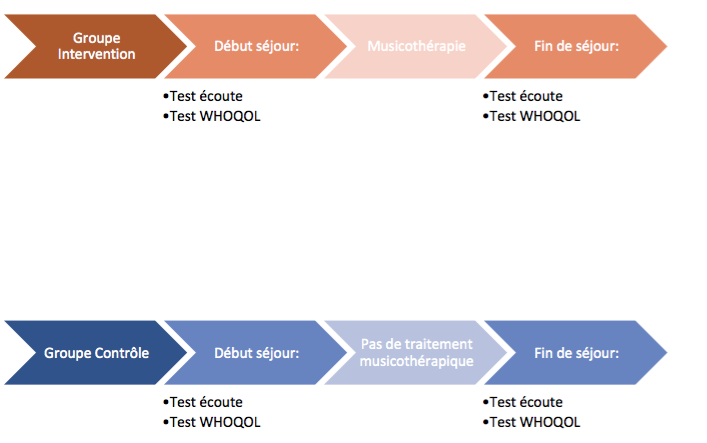
\includegraphics[width=1\linewidth]{images/Groupecontrole.png}
\caption[Schéma du déroulement]{Déroulement de l'étude avec GM et GC}

%\label{groupecontroleimage1}
\end{figure}

 \subsection{Procédure}
Chaque participant du groupe GM et GC va faire en entrée et en sortie de
clinique, après environ 4 semaines, un
          test avec questionnaire  WHO QOL. (GM ayant suivi une musicothérapie active et/ou réceptive (1x par
        semaine).\footnote{Voir Fig. 4.1.}
          Chaque test d'écoute dure
        70 à 90 minutes, fait 2x (pré/post-thérapie) et
        suivi du questionnaire WHOQOL (2x10') rempli par le
        patient lui-même.

Sur \textbf{44 tests d'écoute} réalisés pour \textbf{GC et GM},
      nous avons décompté\textbf{ 30 tests} valides qui serviront de
     comparatif dont \textbf{16} pour
     GM, groupe de musicothérapie et \textbf{14 tests d'écoute} pour GC, le groupe
     contrôle.

\begin{figure}
\centering
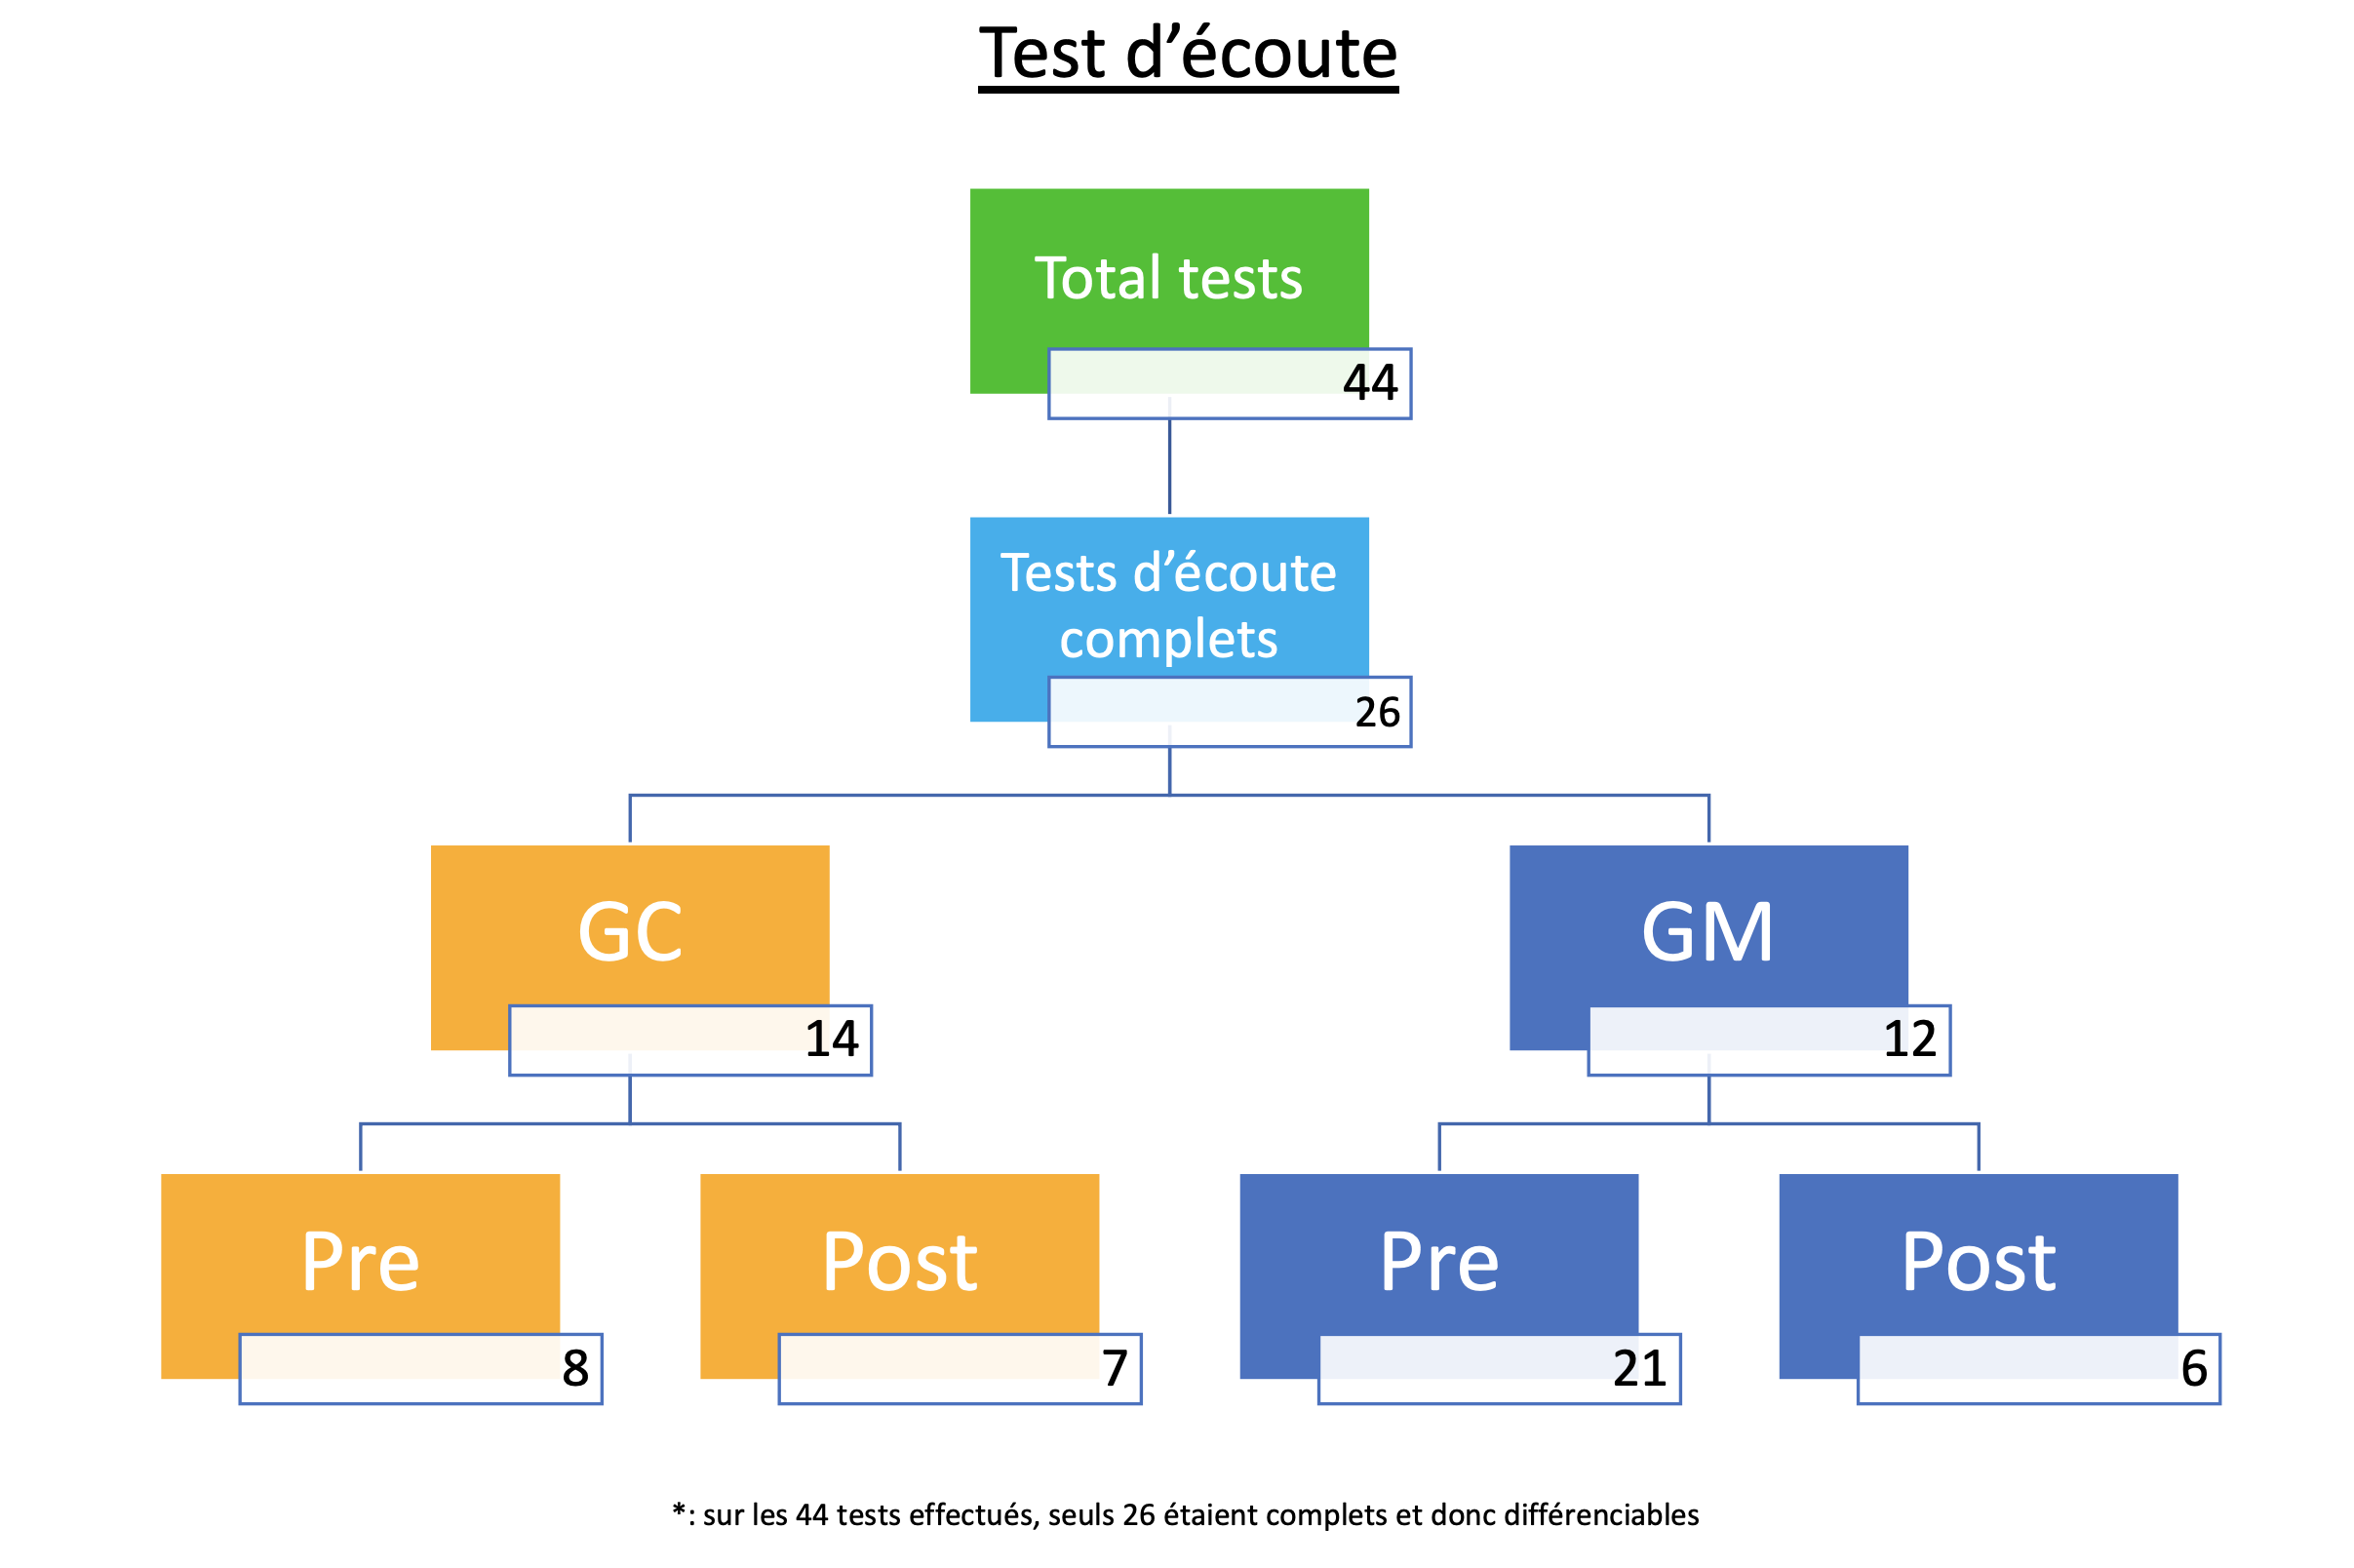
\includegraphics[width=1\linewidth]{images/graphiques/Testecoute.png}
\caption{Nombre de tests d'écoute avec GM et GC}

%\label{groupecontroleimage1}
\end{figure}



     \begin{figure}
     \centering
     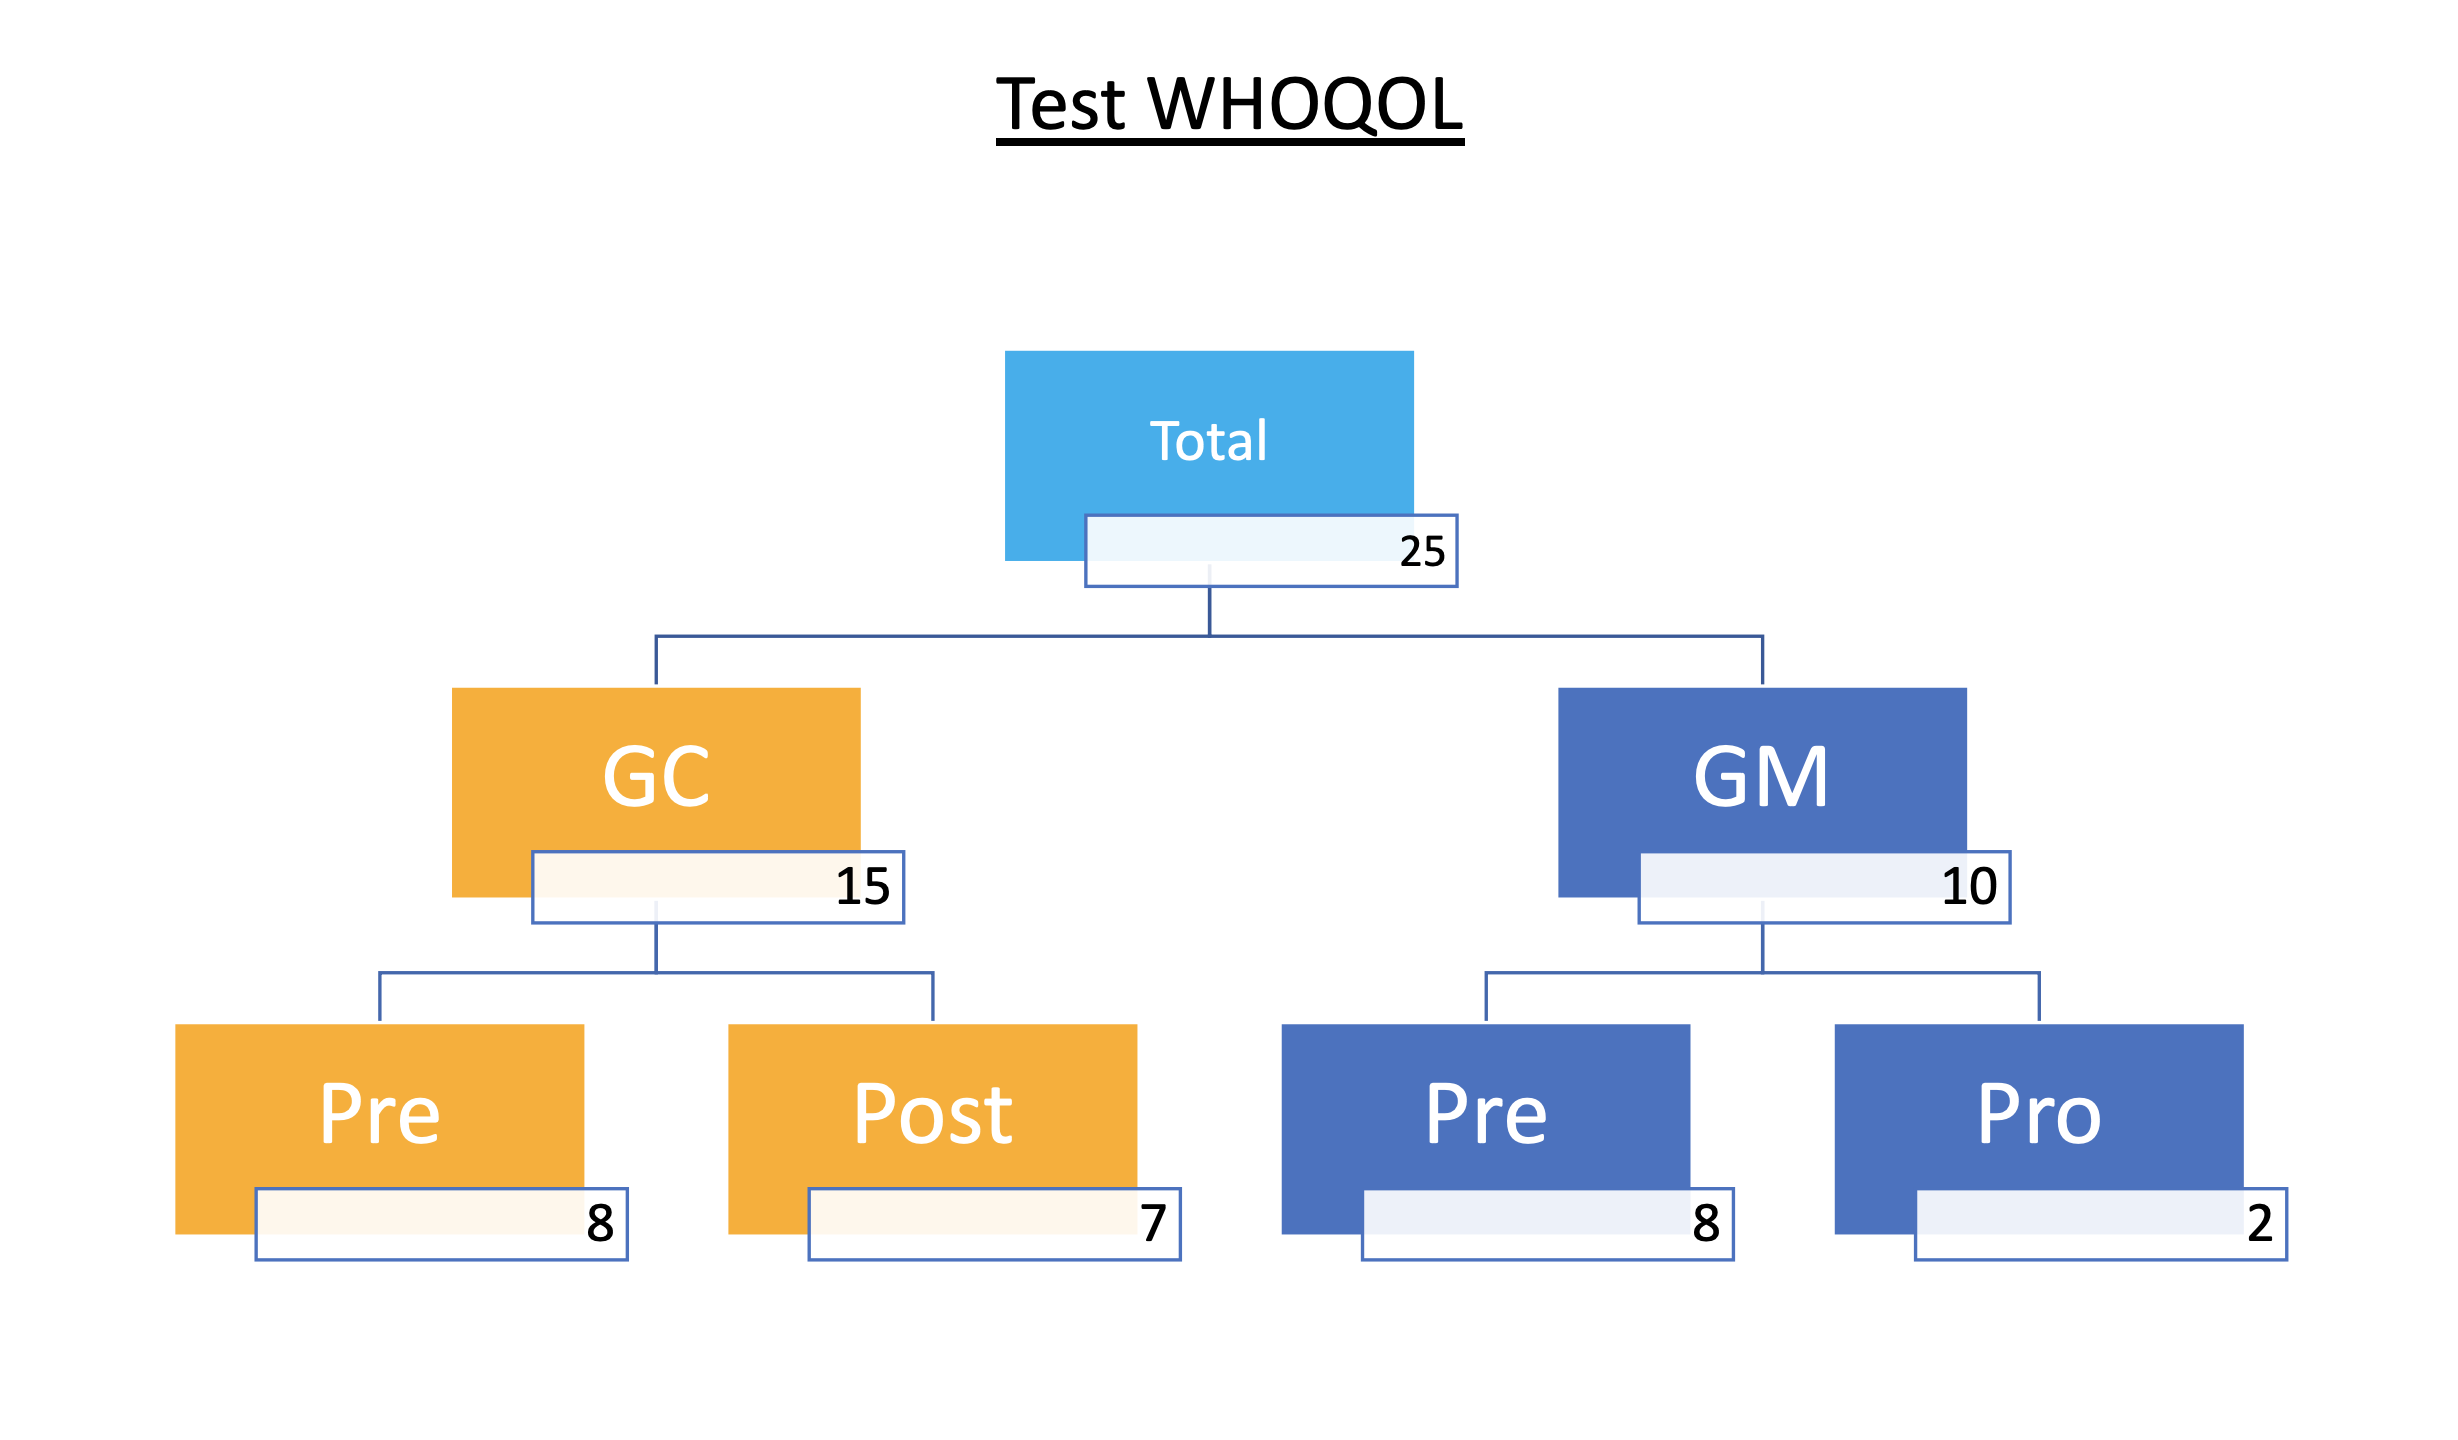
\includegraphics[width=1\linewidth]{images/graphiques/TestWQ.png}
     \caption{Nombre de WHO QOL avec GM et GC}
\end{figure}


Sur \textbf{25 questionnaires WHO QOL}, il y a \textbf{10 pour GM} remplis
avec 8 pré- et seulement 2
     post- thérapies; et \textbf{15 pour GC} dont 8 pré-
     et 7 post-thérapie.
      Nous avons dans l'ensemble un total de \textbf{9 questionnaires} pour le
     comparatif des 2 groupes réunis.


\textbf{ Pathologie des groupes}: Les patients ont été répartis en deux groupes sans différenciation de
 leur pathologie. Nous avons conscience d'avoir mélangé des symptomatologies qui
 toutefois paraissent
 sous-tendues par
                                               certains mécanismes
                                               similaires dont le
                                               noyau commun est une
                                              \textbf{difficulté de
                                               régulation des
                                               émotions},
                                               s'exprimant par une
                                               humeur négative.
                                               Il convient ici de mentionner que, en vue de la taille réduite des échantillons, il n'est pas
pertinent de se lancer dans une analyse purement
quantitative.

\section{Hypothèses opérationnelles}

Il s'agit ainsi d'une étude mixant le \textbf{quantitatif  et le
  qualitatif}.
En procédant toujours en amont et en aval, --pré/postpostthérapie--, nous
avons fait l'obtention de :
\begin{enumerate}

  \item la \textbf{moyenne} \textbf{des seuils
  auditifs de la c.a.} de l'oreille \textbf{droite} et de
  l'oreille \textbf{gauche} de \textbf{chaque patient}
  \item la \textbf{moyenne} \textbf{des seuils
  auditifs de la c.o.} de l'oreille \textbf{droite} et de
  l'oreille \textbf{gauche} de \textbf{chaque patient}
\item la \textbf{comparaison des dessins des différentes courbes}
\item le \textbf{nombre de croisements entre c.a. et c.o}
\end{enumerate}.
Nous avons illustré
plusieurs exemples.
Ainsi, après avoir
fait une comparaison des dessins des différentes courbes et
décompté le nombre des croisements, l'ensemble des résultats a été analysé et comparé, puis mis en corrélation avec ceux du\textbf{
  WHO QOL}.

Qu'il s'agisse des tests ou des questionnaires, nous avons choisi de
simplifier les \textbf{résultats} sous forme de signes
mathématiques, $+$, $=$, $-$ avec les significations suivantes.
Avec les \textbf{tests d'écoute}:
\begin{enumerate}
\item$+$   : amélioration, modification;  rapprochement significatif à la courbe dite idéale.
\item$=$   : amélioration insignifiante, correspond à : $+/-$, (si c.a. $ + $ et c.o. $-$, ou vice-versa).

\item$-$   : pas d'amélioration et pas/trop peu  de modification, inversion
des courbes (c.o. supérieure à c.a.).

  Avec les \textbf{croisements}, les chiffres des 2 tests pré/post
  nous permettent d'obtenir une comparaison:
  \item Plus petit est le nombre, meilleur est le résultat, ce qui correspond à un signe positif : $+$.
\item Dans le
  cas contraire, ce sera un signe négatif: $-$.

\end{enumerate}


 \section{Test d'ECOUTE: comparatif pré/post-thérapie }
Avec les tests d'écoute, nous
allons donc prendre en compte, l'observation par \textbf{comparaison graphique des différentes
  courbes}

\begin{enumerate}
 \item   les \textbf{seuils} auditifs --moyenne
représentée sous forme de la  \textbf{courbe aérienne}
\item   les \textbf{seuils} auditifs --moyenne
représentée sous forme de la \textbf{courbe osseuse}
\item le nombre de
\textbf{croisements}.\footnote{Cf. Ch. 3 A. Tomatis p. 26: les distorsions}

\end{enumerate}


%\textbf{Index courbe idéale aérienne et osseuse}:
%La moyenne chiffrée de la courbe aérienne: 1,3
%La moyenne chiffrée de la courbe osseuse: 3,11
Remarque: nous n'avons pas pu ici montrer l'intégralité des tests d'écoute, mais ceux-ci se trouvent à disposition sur demande et en toute confidentialité.
%Notons que nous avons évidemment fait l'ensemble de l'analyse.
Nous présentons ici un échantillonnage.

  \subsection{Groupe CONTRÔLE: Observation des tests d'écoute de 3 patients.}


      \textbf{Groupe Contrôle : 3 patients}
  \paragraph{ A. Patient Br.:}
  \begin{figure}[ht]
\centering
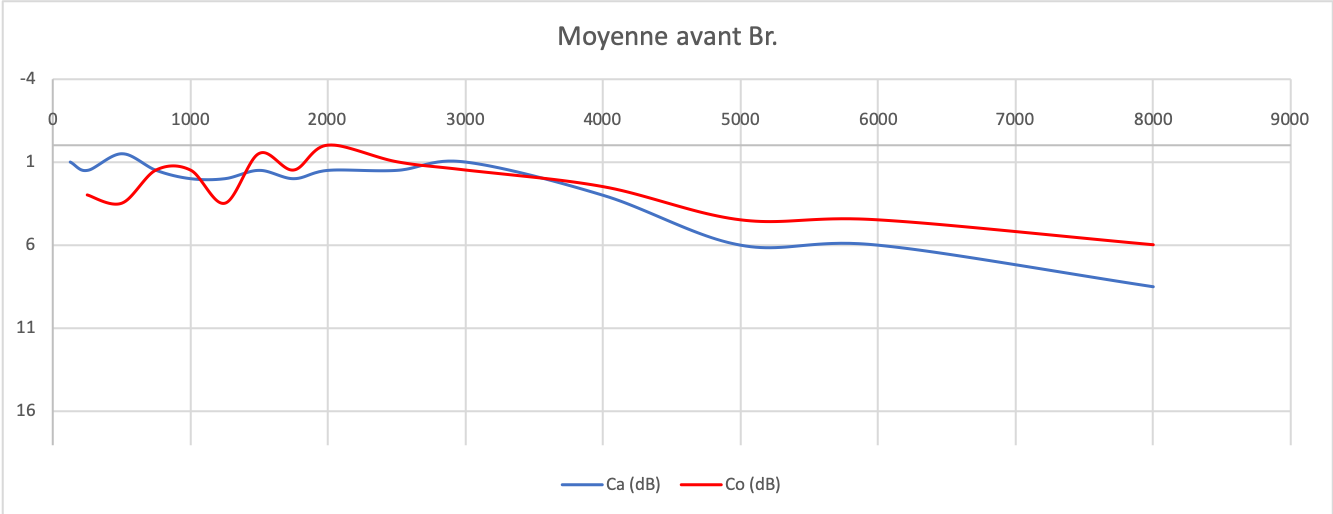
\includegraphics[width=0.7\linewidth]{images/graphiques/bru_pre.png}
\caption[Moyenne OG+OD]{Premier test Br.}

%\label{groupecontroleimage1}
\end{figure}



 \begin{figure}[th]
\centering
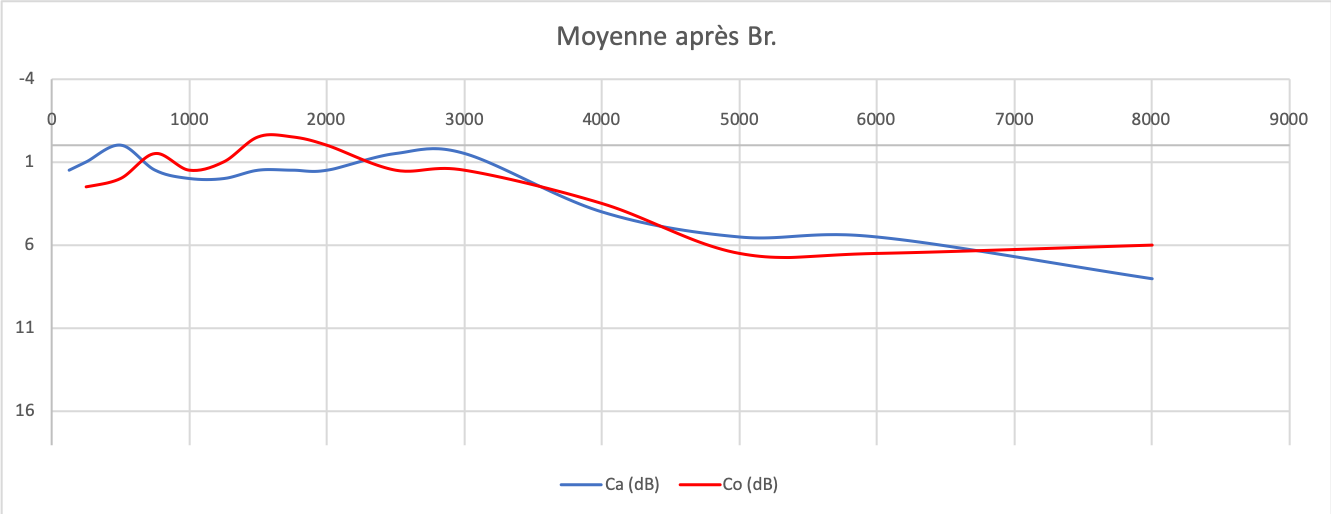
\includegraphics[width=0.7\linewidth]{images/graphiques/bru_post.png}
\caption[Moyenne OG+OD]{Second test Br.}

%\label{groupecontroleimage1}
\end{figure}

	\begin{enumerate}
 		\item  c.a.: pas de modification, augmentation des
                  seuils: $-$
 		\item  c.o.: redressement des seuils: $+$
 		\item  croisements: $5/4$ : $+$ : ce qui signifie:  5 croisements lors du 1°test// 4 croisements lors du 2° test= nous avons 1 croisement en moins, donc le résultat est considéré comme positif en fin
                  de séjour.
                \end{enumerate}

                \textbf{  Conclusion:  -    +    +       :  +}




\paragraph{B. Patient Sch.:}

	\begin{enumerate}

 		\item : c.a.: pas de modification, très légère augmentation des
                  seuils: +/-
 		\item : c.o.: a passé sous c.a., modification des seuils: +
 		\item : croisements: 2/2 :     =
                   \end{enumerate}
 \textbf{  Conclusion:  +/-    +    =        :  =}

\begin{figure}[th]
\centering
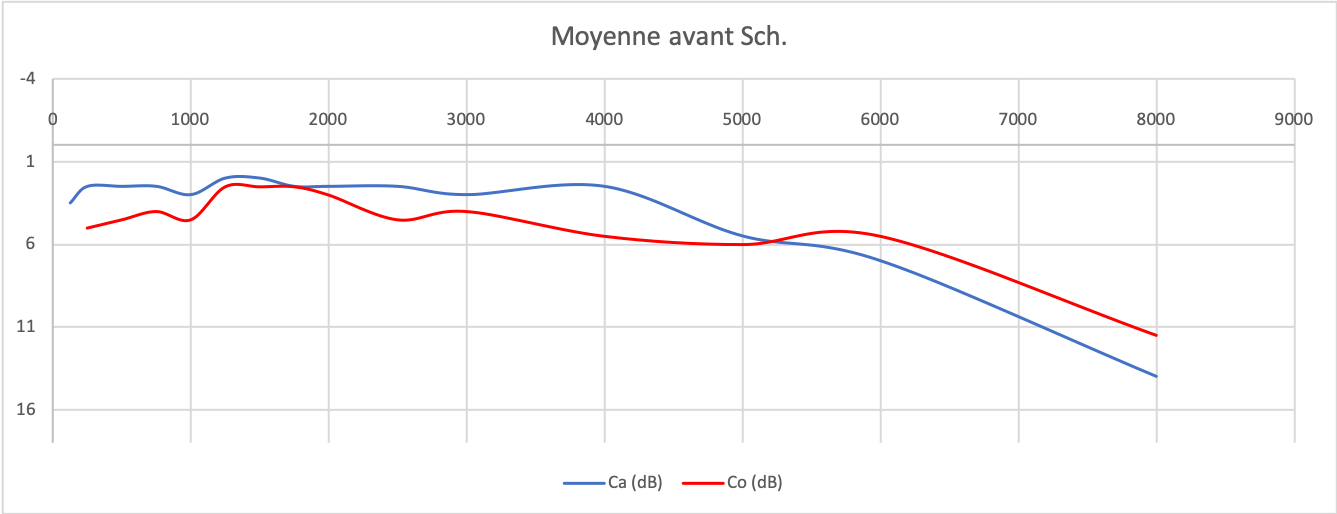
\includegraphics[width=0.7\linewidth]{images/graphiques/schaff_pre.png}
\caption[Moyenne OG+OD]{Premier test Sch.}

%\label{groupecontroleimage1}
\end{figure}


         \begin{figure}[th]
\centering
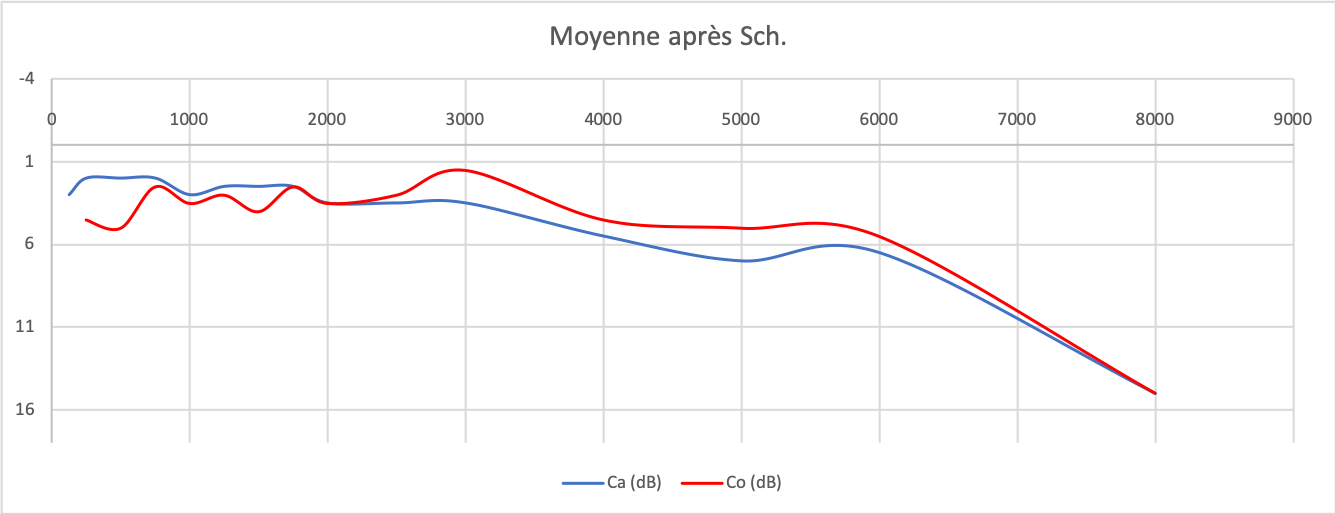
\includegraphics[width=0.7\linewidth]{images/graphiques/schaff_post.png}
\caption[Moyenne OG+OD]{Second test Sch.}

\label{groupecontroleimage1}
\end{figure}


\paragraph{C. Patient Wal.:}



\begin{figure}[th]
\centering
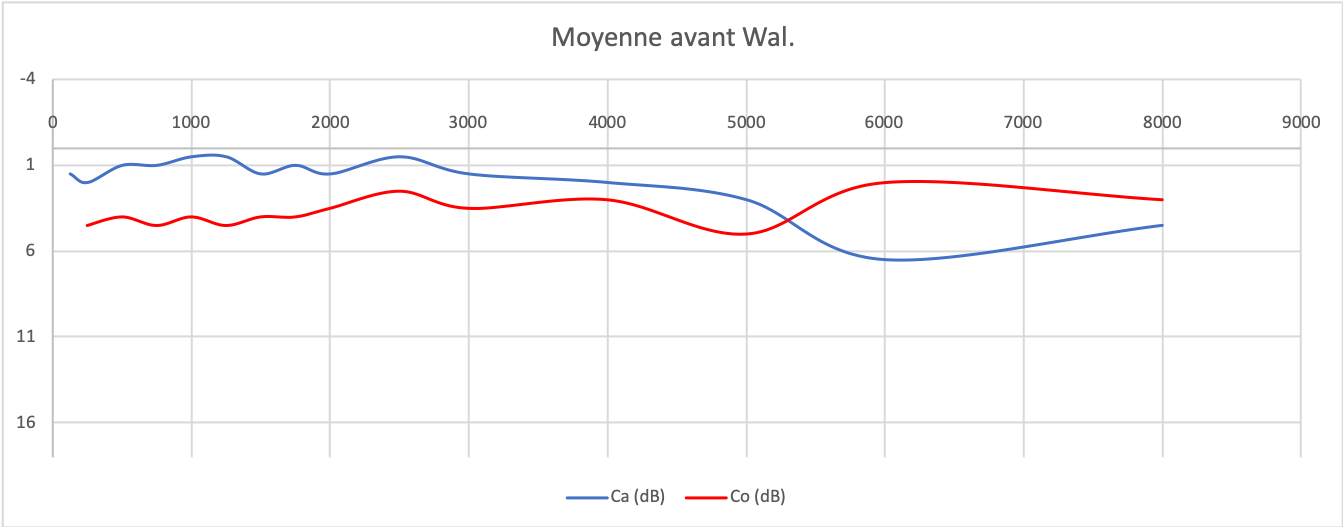
\includegraphics[width=0.7\linewidth]{images/graphiques/wal_pre.png}
\caption[Moyenne OG+OD]{Premier test Wal.}

%\label{groupecontroleimage1}
\end{figure}

	\begin{enumerate}

 		\item : c.a.: peu de modification: =

 		\item : c.o.: reste dominante, tentative de rapprochement de c.a.: -
 		\item : croisements: 1/3 :  -

                \end{enumerate}

                \textbf{ Conclusion:  $= -  -        : -$ }

               \begin{figure}[th]
\centering
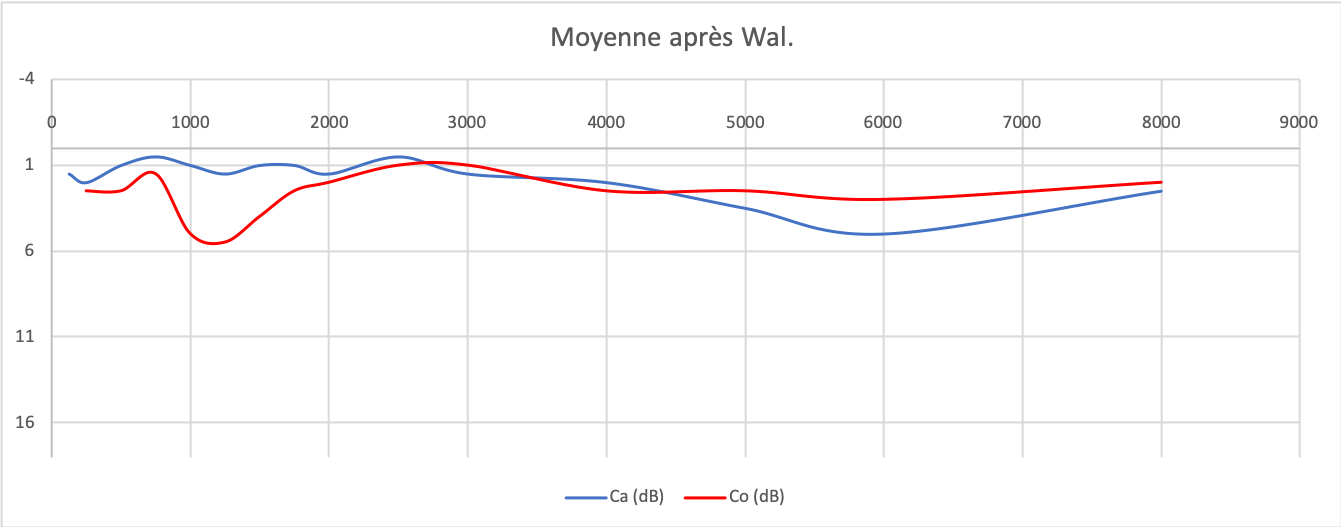
\includegraphics[width=0.7\linewidth]{images/graphiques/wal_post.png}
\caption[Moyenne OG+OD]{Second test Wal.}

\label{groupecontroleimage1}
\end{figure}
\subsection{Groupe MUSICOTHéRAPIE: Observation des tests d'écoute de 3 patients}
  \textbf{Groupe de Musicothérapie: 3 patients}

\paragraph{ A. Patient Sw.:}



 \begin{figure}[th]
\centering
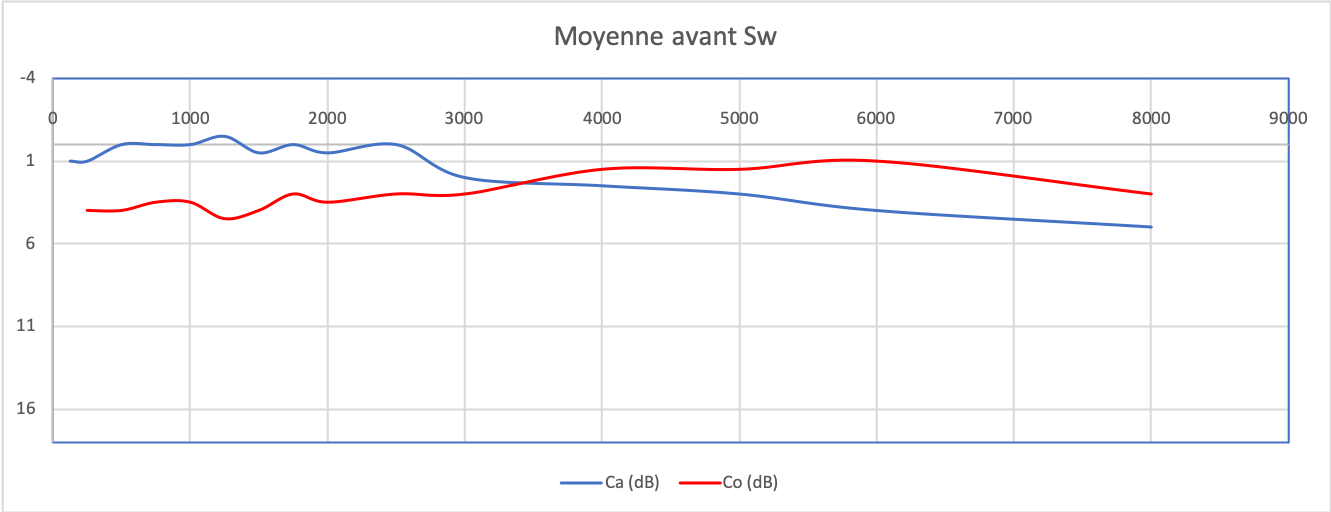
\includegraphics[width=0.7\linewidth]{images/graphiques/sw_pre.png}
\caption[Moyenne OG+OD]{Premier test Sw.}

%\label{groupecontroleimage1}
\end{figure}

	\begin{enumerate}

 		\item : c.a.: pas de modification: = %  1,27/1,27

 		\item : c.o.: redressement et rapprochement,
                  relèvement des seuils: -       %  3,07/3,39
 		\item : croisements: 1/3 :  -

                \end{enumerate}

                \textbf{  Conclusion:  = +  -        : ``=''}

                \begin{figure}[th]
\centering
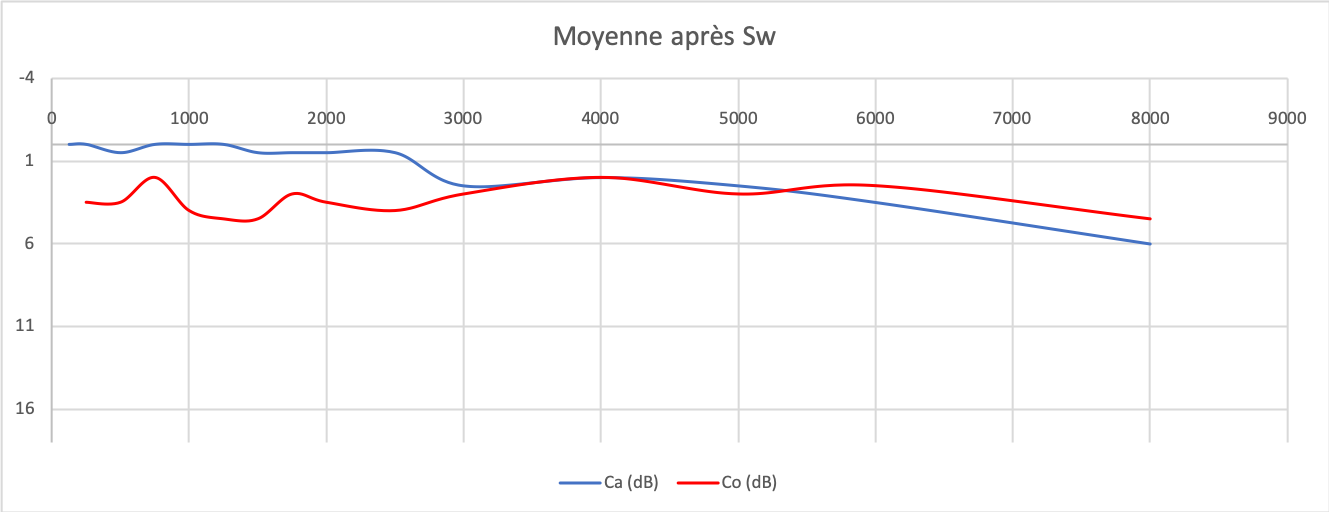
\includegraphics[width=0.7\linewidth]{images/graphiques/sw_post.png}
\caption[Moyenne OG+OD]{Second test Sw.}

%\label{groupecontroleimage1}
\end{figure}




\paragraph{B. Patient Cav.: }

(pas de WOQOL fin de séjour)


\begin{figure}[th]
\centering
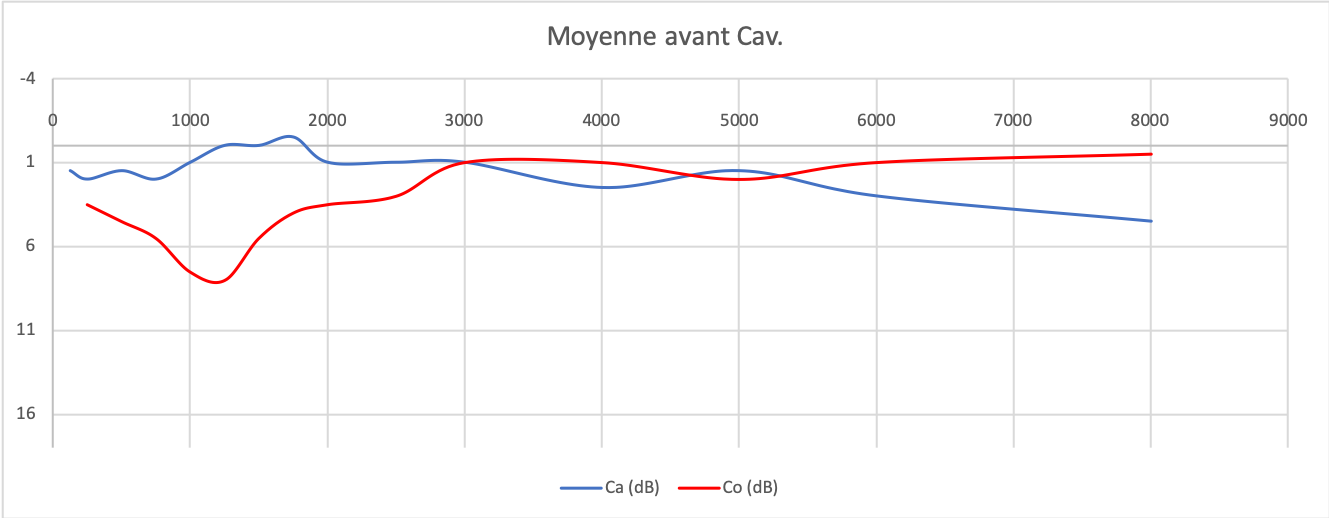
\includegraphics[width=0.7\linewidth]{images/graphiques/cav_pre.png}
\caption[Moyenne OG+OD]{Premier test Cav.}

%\label{groupecontroleimage1}
\end{figure}

	\begin{enumerate}

 		\item : c.a.: redressement: +

 		\item : c.o.: redressement et rapprochement, relèvement des seuils: +
 		\item : croisements: 3/1 :  +

                \end{enumerate}

                \textbf{  Conclusion:  + + +       : ``+''}

                \begin{figure}
\centering
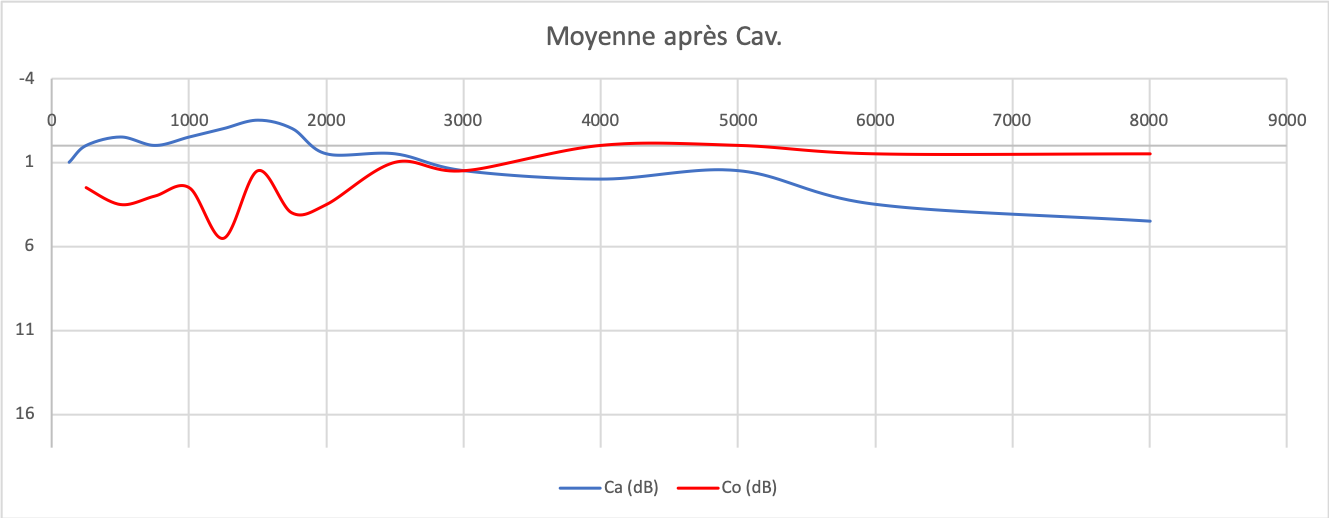
\includegraphics[width=0.7\linewidth]{images/graphiques/cav_post.png}
\caption[Moyenne OG+OD]{Second test Cav.}

%\label{groupecontroleimage1}
                \end{figure}




               \paragraph{ C. Patient M.:}


	\begin{enumerate}

 		\item : c.a.: redressement: : +   % 6,43/6,03

 		\item : c.o.: redressement et rapprochement,
                  relèvement des seuils:  +     %6,25/5,85:
 		\item : croisements: 3/3 :  =

                \end{enumerate}

                \textbf{  Conclusion:  +  +  =     : ``+''}

                \begin{figure}[th]
\centering
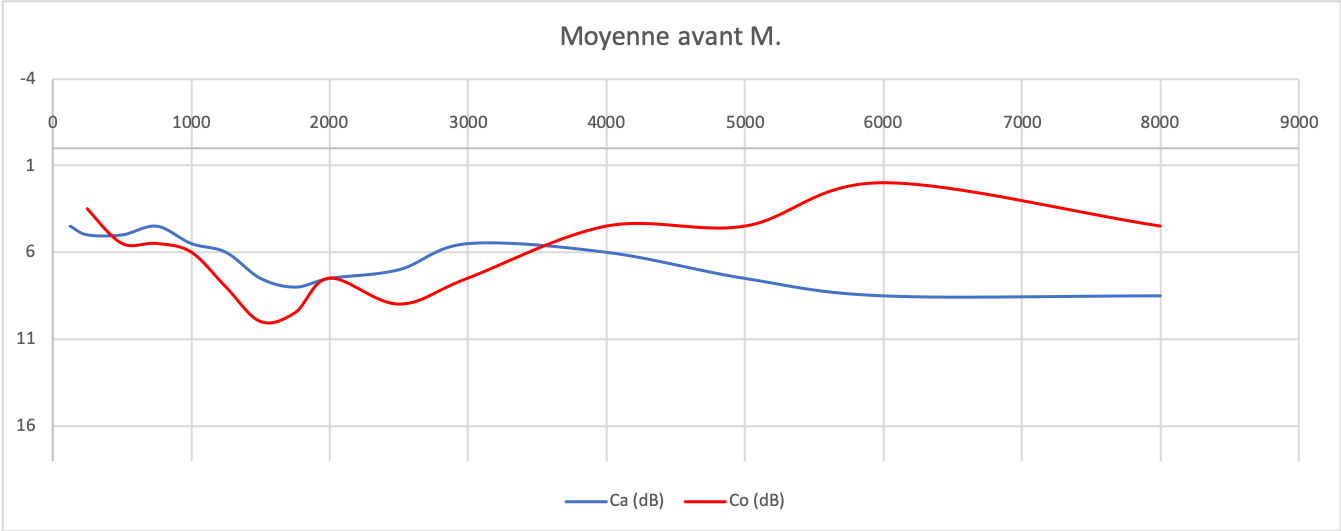
\includegraphics[width=0.7\linewidth]{images/graphiques/m_pre.png}
\caption[Moyenne OG+OD]{Premier test M.}

%\label{groupecontroleimage1}
\end{figure}


                        \begin{figure}[th]
\centering
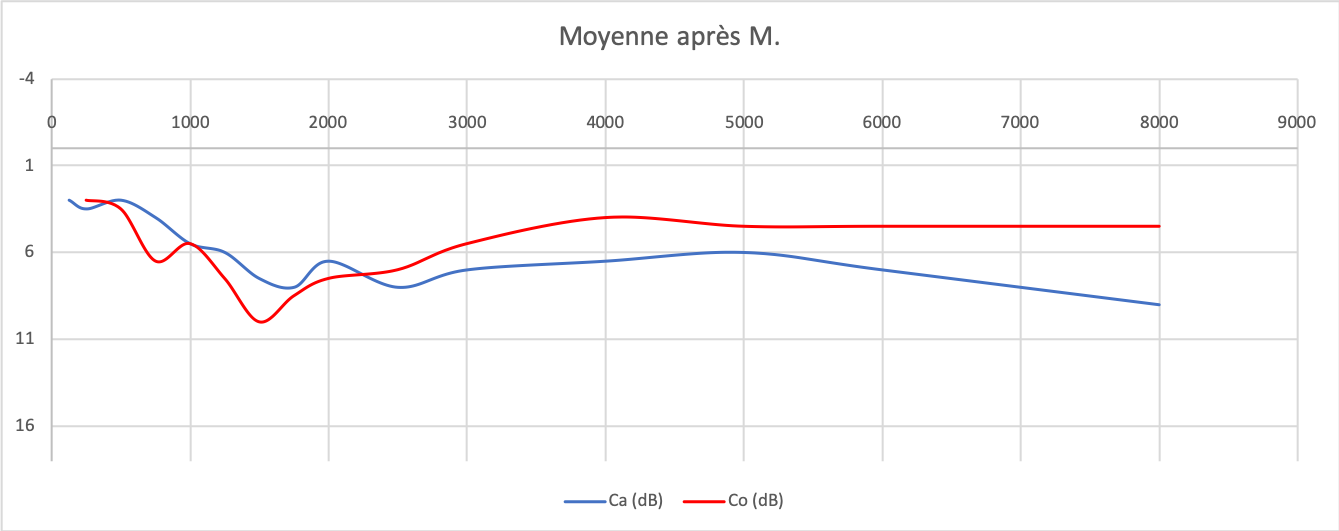
\includegraphics[width=0.7\linewidth]{images/graphiques/m_post.png}
\caption[Moyenne OG+OD]{Second test M.}

%\label{groupecontroleimage1}
\end{figure}




\subsection{Test d'ECOUTE: résultats du comparatif pré/post-thérapie}

\textbf{Conclusions générales}:

             Nous nous trouvons
           en présence de deux groupes, un groupe de contrôle et un
           groupe de musicothérapie ayant le même type de
           pathologie --difficulté de régulation des émotions-- .


           Nous constatons tout d'abord que l'écoute est quantifiable.
           D'autre part, il existe bien
          une \textbf{modification de l'écoute pré -- et post -- traitement}.


          Ensuite, il est à observer que
          cette modification est nettement plus marquée
          pour GM, groupe de musicothérapie, qui a un résultat positif.


          \textbf{GM: ``+''}.


Par contre,  pour le groupe de contrôle, GC, le résultat est mitigé, il correspond au signe d'égalité et n'apporte aucune vraie modification.

          \textbf{GC:  ``='' ou +/-}.


        D'autre part, remarquons que les données quantitatives observables dans ces graphiques semblent aller dans le
sens de  l'étude faite par le
CNRS (Cf. Ch. Introduction, p. 16) \autocite{affectiveDisorders} réalisée à partir des seuils auditifs, à savoir
les patients souffrant de troubles post-traumatiques souffrent d'un
\textbf{appauvrissement caractéristique de fréquences.}

\section{Questionnaires WO - QOL : comparatif pré/post-thérapie }


\begin{figure}[tbh]
\centering
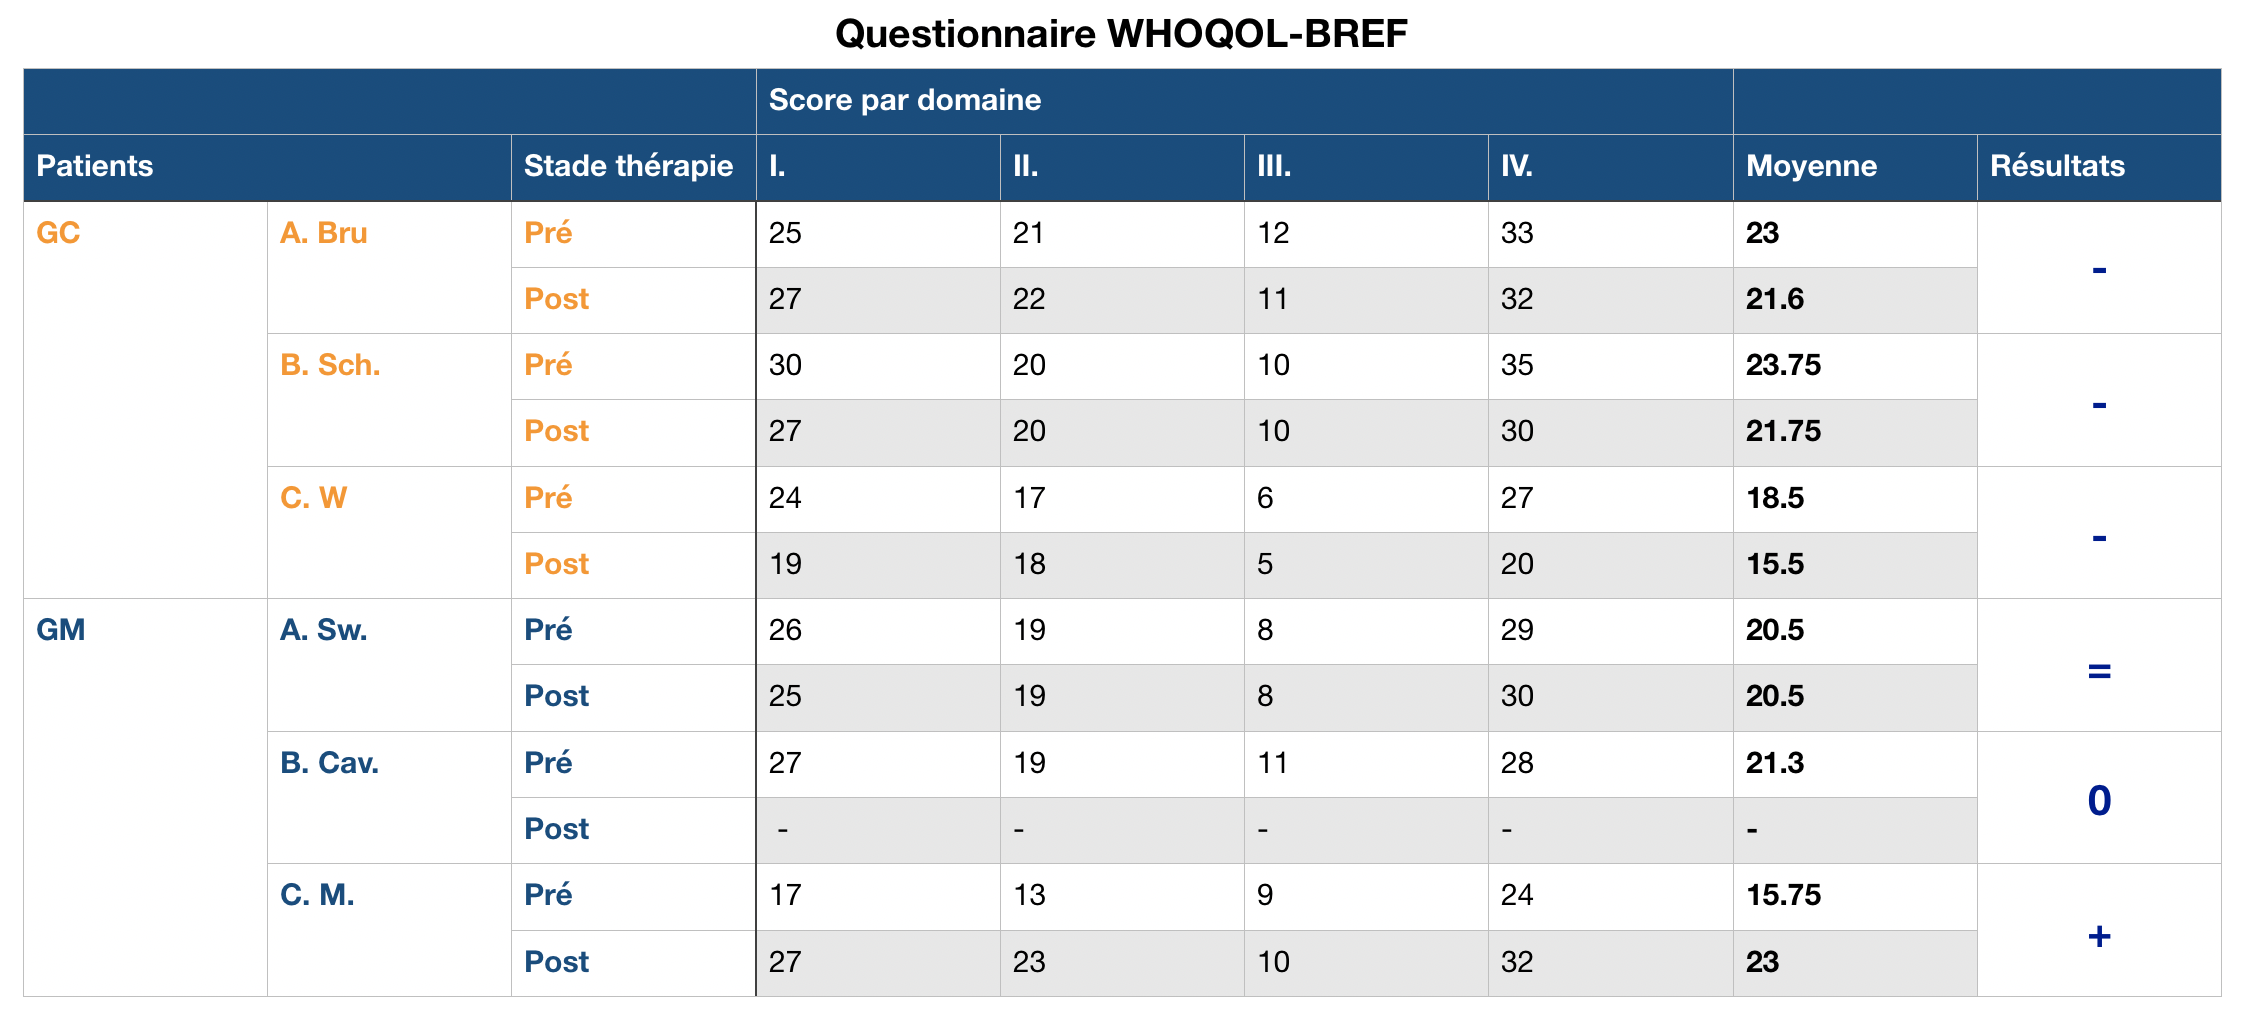
\includegraphics[width=1.2\linewidth]{images/graphiques/questionnaire_wq.png}
\caption[Questionnaire WHOQOL-BREF]{GM/GC - Pré/Post avec la moyenne des scores par domaine}

%\label{groupecontroleimage1}
\end{figure}
Voici à présent le schéma (Fig. 4.16.) représentant la
moyenne pré -- et post -- traitement, calculée pour chaque patient, des scores
des 4 domaines.
%Les chiffres ont été obtenus à partir des 4
%domaines, avec le pré/post-séjour.
Remarque: si, par comparaison, le chiffre post-séjour est plus élevé
que celui du
pré-séjour, le résultat final obtenu est considéré comme
positif. Par conséquent, nous
observerons soit un score négatif, positif ou égal (sans changement).


Nous avons mis en détail  \textbf{à titre d'exemple } 3 patients du GC et 2 du GM
( les seuls valides pour la comparaison, le patient CAV mentionné comme preuve de l'inexistence du questionnaire rempli en fin de thérapie) afin d'être le plus clair possible
dans notre façon de procéder.
A la fin, nous avons illustré en couleur (Fig. 4.18 et 4.19.) les
résultats finaux des deux groupes au complet avec 2 schémas
comparatifs.
\subsection{Groupe CONTRÔLE: observation des résultats avec 3 patients}
%\paragraph{ GC: Représentation des résultats avec 3 patients du groupe contrôle:}

\begin{enumerate}
\item : A. Patient Br.:  25/27 - 21/22 - 12/11 - 33/32 =  ''-''

          Résultat: 21,6 contre 23 pré-traitement,  ce qui
        correspond au signe négatif.
      \item : B. Patient Sch.: 30/27 - 20/20 -  10/10 - 35/30 = ''-''

         Résultat: 21,75 contre 23,75 pré-traitement, ce qui
        correspond au signe négatif.

 		\item :  C. Patient Wal. : 24/19 -  17/18 - 6/5 -
                  27/20 =  ''-''

                  Résultat: 15,5 contre 18,5 pré-traitement, ce qui
        correspond au signe \textbf{négatif: ''-''}.
 	\end{enumerate}


       \textbf{ Conclusion}: les résultats sont \textbf{négatifs}.
        Ces exemples confirment
        le ressenti subjectif moyen de l'ensemble des patients
        GC post-traitement, comme représenté à la Figure 4.18.
        \subsection{Groupe MUSICOTHéRAPIE: observation des résultats avec 2 patients}

       %\paragraph{ GM: Représentation de résultats avec 2 patients du groupe de musicothérapie}

\begin{enumerate}
 		\item : A. Patient Sw. : 26/25 - 19/19 - 8/8 - 29/30 =  ''=''



  Résultat: 20,5 contre 20,5 pré-traitement, ce qui
        correspond au signe égal.



 		\item : B. Patient M.: 17/27 - 13/23 -  9/10 - 24/32 = ``++''

              Résultat: 23 contre 15,75 pré-traitement, correspondant
              au signe \textbf{positif: ""+""}
            \end{enumerate}
 \textbf{ Conclusion}: les résultats sont \textbf{positifs}.


                 Ainsi,  GM s'exprime
                 \textbf{positivement}
                 sur l'ensemble du séjour en clinique.

                 \subsection{Questionnaires WO - QOL : résultat du comparatif pré/post-thérapie}



\begin{figure}
\centering
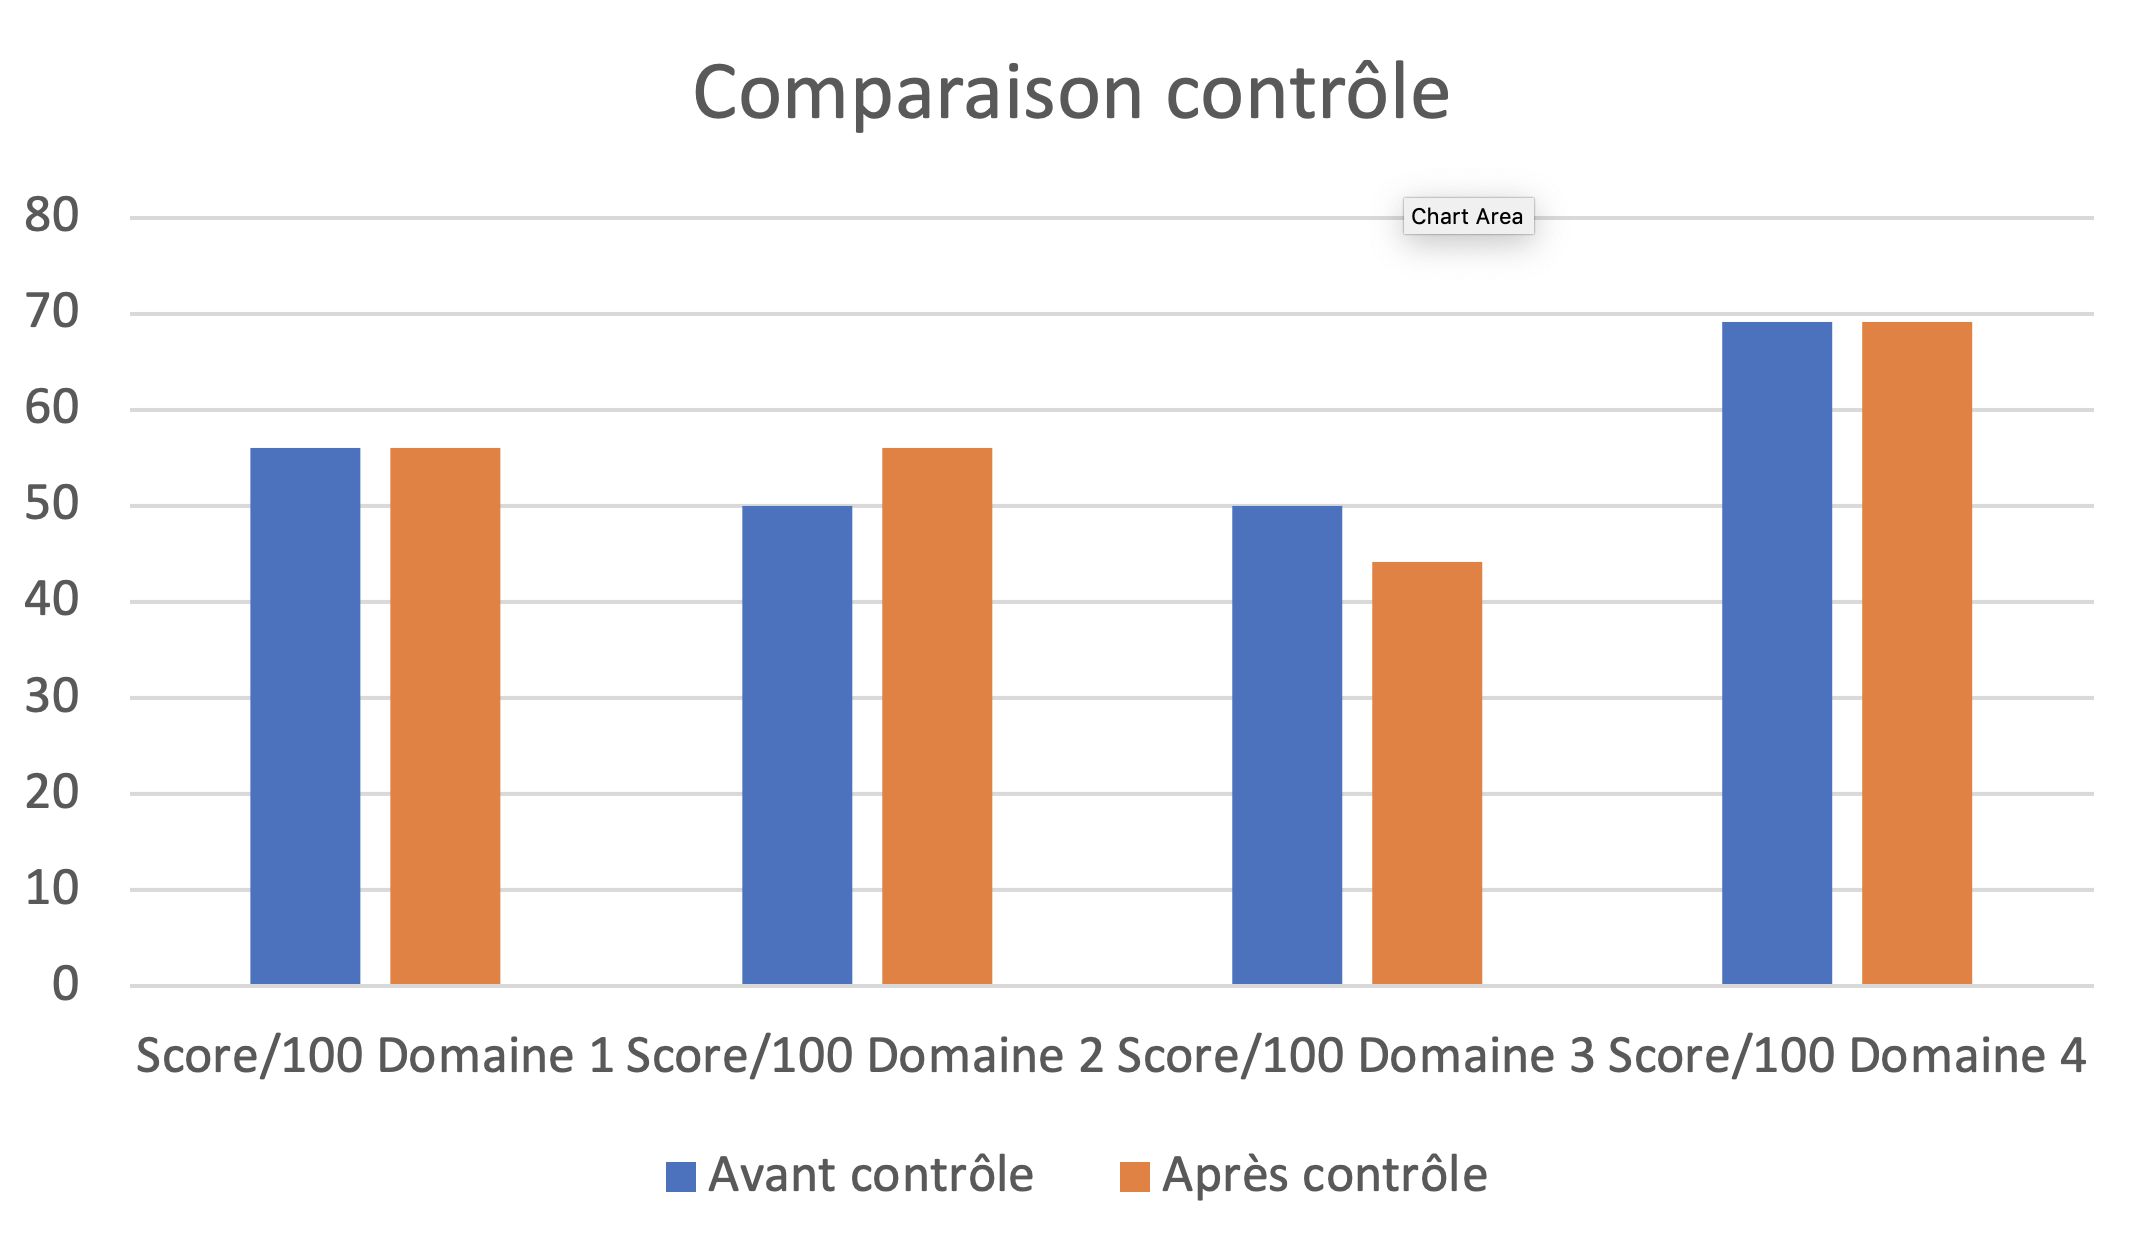
\includegraphics[width=1.0\linewidth]{images/Compcontrole.png}
\caption[Schéma du déroulement]{WHO QOL:  GC. Comparatif pré/post-traitement}

%\label{groupecontroleimage1}
\end{figure}

\begin{figure}
\centering
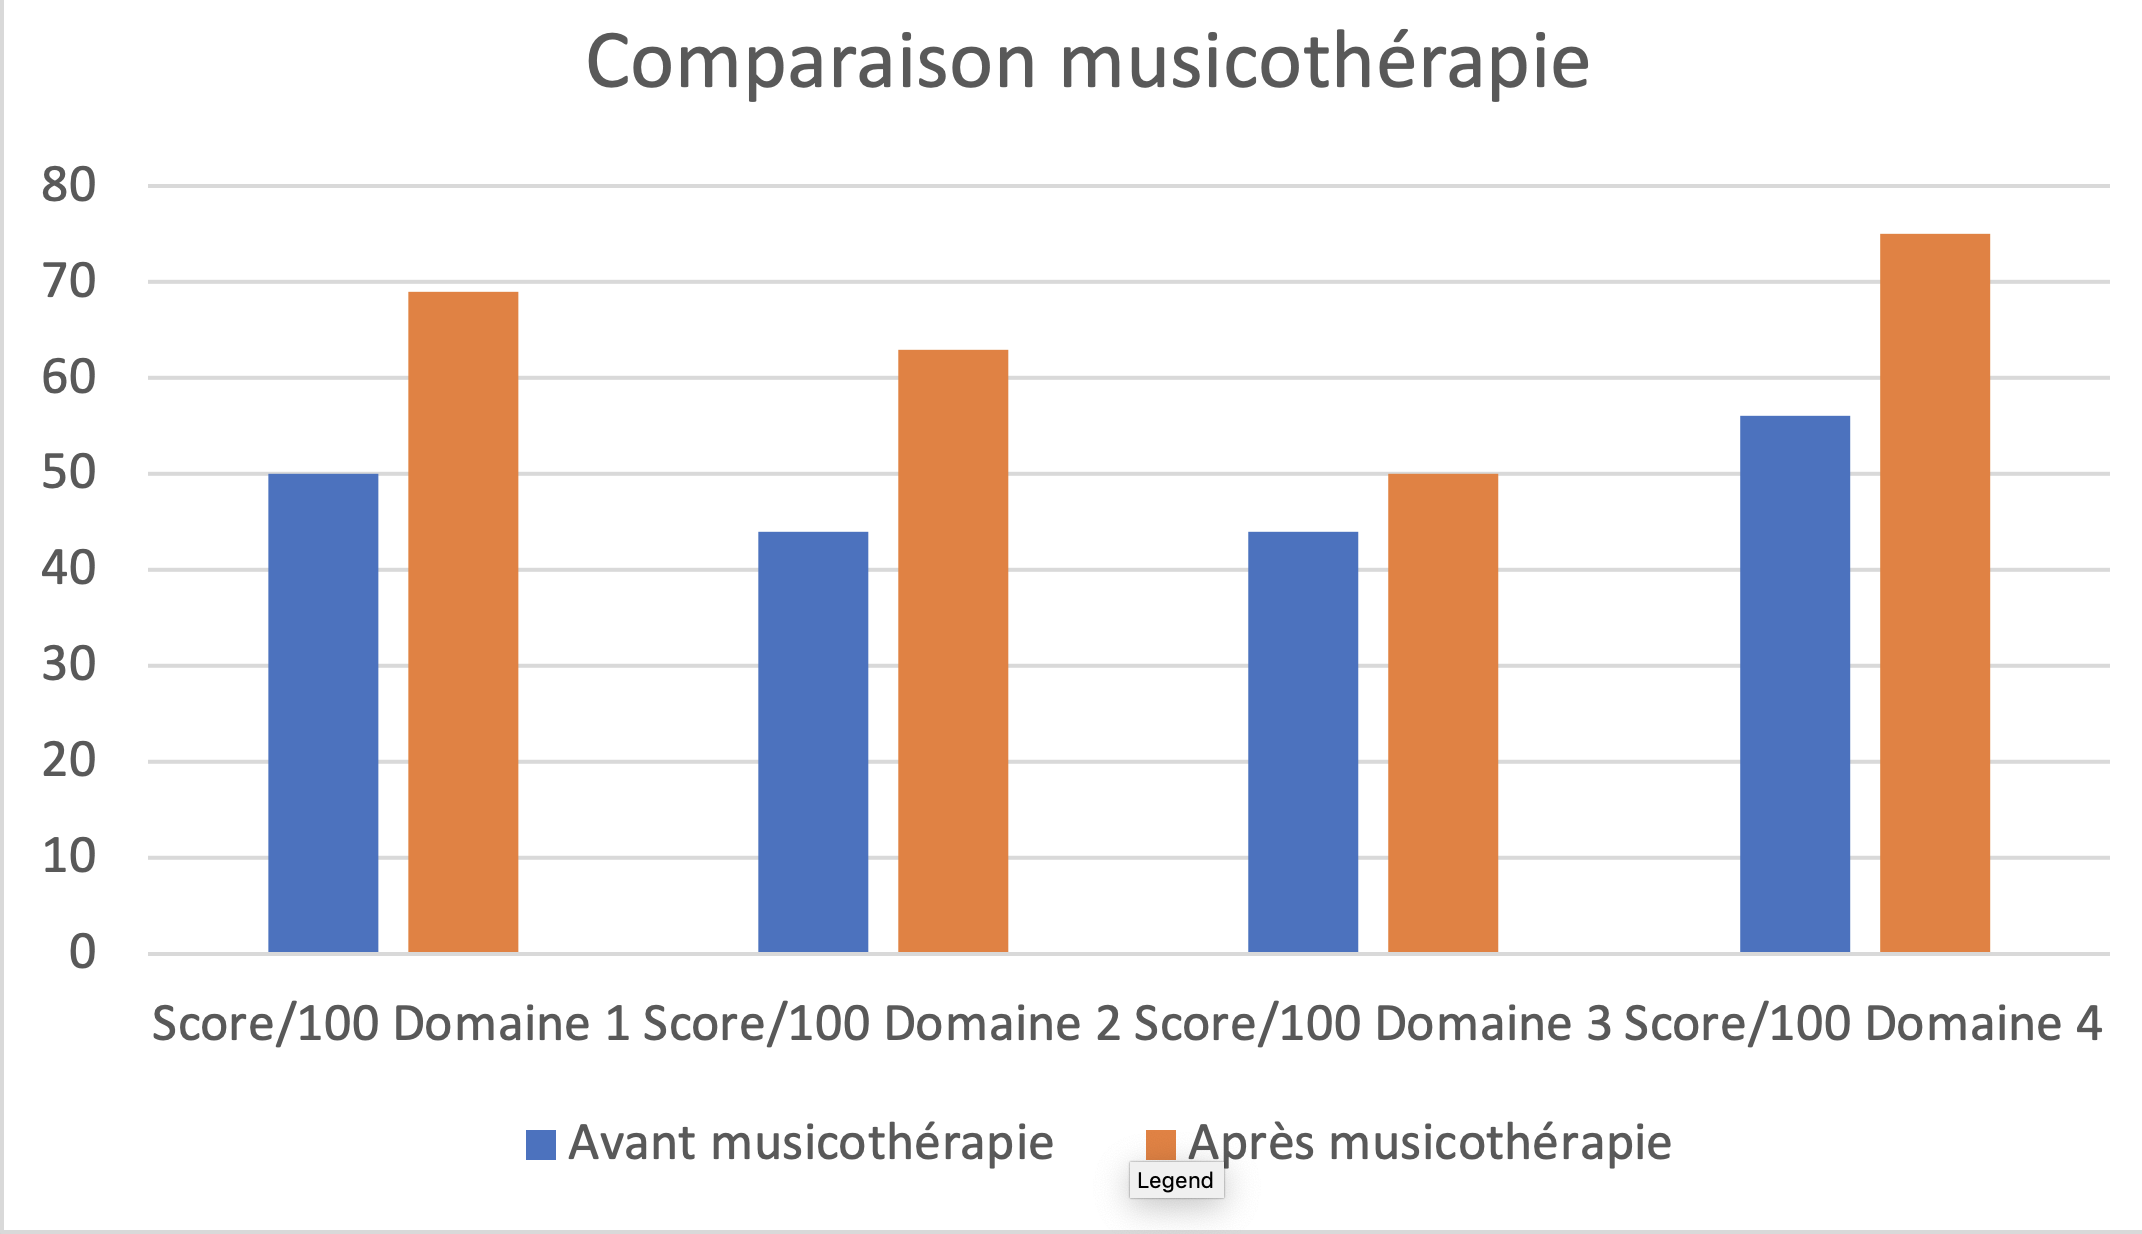
\includegraphics[width=1.0\linewidth]{images/Compmusico.png}
\caption[Schéma du déroulement]{ WHO QOL: GM. Comparatif pré/post-traitement }

%\label{groupecontroleimage1}
\end{figure}


Nous avons obtenu un comparatif graphique  des résultats des questionnaires
pré/post-traitement du groupe de contrôle, puis du groupe de musicothérapie,
graphiques se trouvant sous les Fig. 4.17 et 4.18.
       En résumé, nous observons que, selon les chiffres obtenus, le ressenti
       subjectif d'amélioration psychique
        des patients suivis en musicothérapie apparait comme
        supérieur.
        De manière générale, l'ensemble des données des deux groupes représentés
        par les graphiques corrobore ce résultat.
        Ces données sont des valeurs indicatives car nous avons conscience que l'échantillonnage ne
        peut pas être représentatif, comme déjà dit plus haut, dû
        notamment à un
        manque de
        questionnaires WH QOL, raisons pour lesquelles nous avons
        restreint le nombre d'exemples WQ présentés ici, pour obtenir
        une parité avec les tests d'écoute et obtenir la
        \textbf{corrélation test d'écoute et questionnaire} qui
        suit:

  \section{Corrélation des résultats des tests d'ECOUTE et des WH QOL avec le Groupe Contrôle et le
    Groupe Musicothérapie:}
\textbf{Groupe Contrôle:} 	          \textbf{ test d'écoute: ``=''   et    WQ: ``-'}


\textbf{Groupe Musicothérapie:}     \textbf{test d'écoute: ``+''      et    WQ: ``+''}


 \begin{figure}[th]
\centering
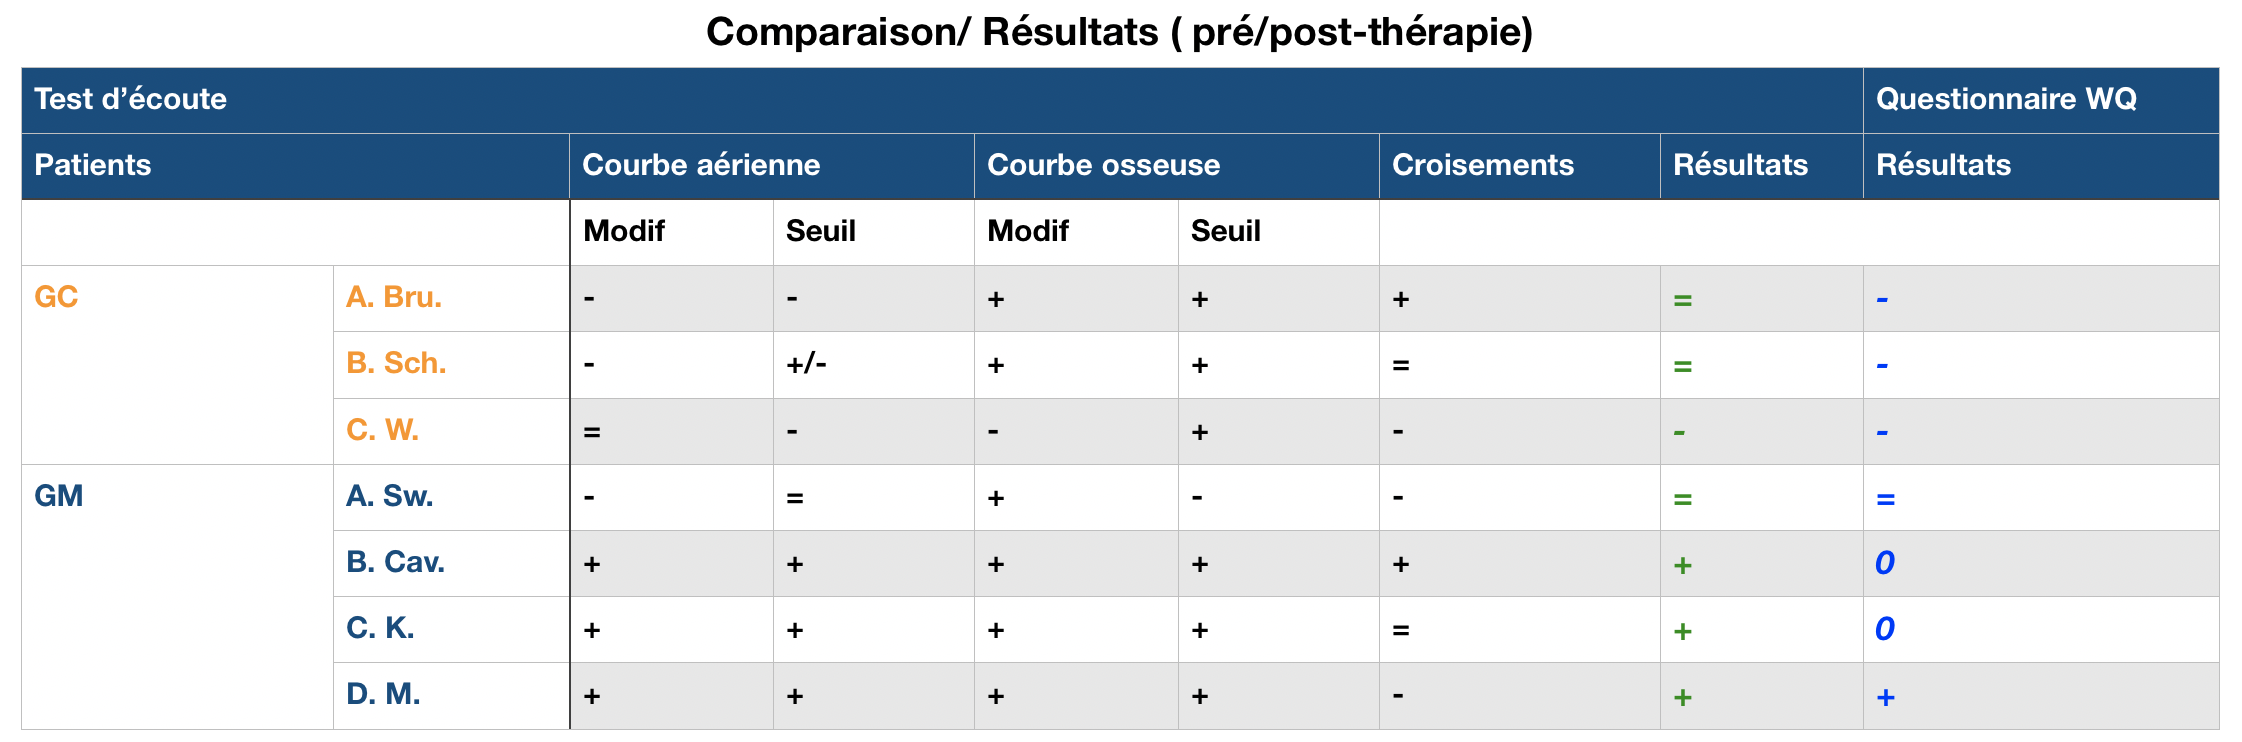
\includegraphics[width=1\linewidth]{images/graphiques/comparaison_pre_post.png}
\caption[Corrélation résultats pré/post]{Comparatif
  pré/post-traitement, WHO QOL, test d'écoute, GM, GC.}

\label{comparaison_pre_post}
\end{figure}


Le résultat final comparatif en corrélation du test d'écoute et du questionnaire WH QOL nous permet
                de relever l'impact positif de la
                musicothérapie sur GM, résultat renforcé
                avec le WQ.


                Pour GC, l'ensemble des résultats sont neutres pour le
                test d'écoute. En ce qui concerne le
                regard des patients sur eux-même avec le WQ, il est
                même négatif. Avec les patients du Groupe de
              Contrôle, nous remarquons, grâce aux tests, une courbe aérienne
              sans modification mais une courbe osseuse plus
              particulièrement réactive. Contrairement à
              ce que le patient pouvait ressentir ou estimer, nous pouvons supposer qu'il y a indication  et attestation d'une amorce de
              processus intérieur et ce, par un autre biais, celui de
              la transformation de son
              écoute.

 Par ailleurs, indistinctement pour les deux
 groupes, il existe ainsi pour le thérapeute des
 suggestions de différentes pistes de travail dans le but de
 solliciter le patient plus spécifiquement en se référant aux
              différentes zones (Cf. Ch. 5. 3, Fig. 5. 1), également zones
 d'élaboration psychique. Ce peut être, par exemple,
              l'expression verbale, si la courbe aérienne est restée
              totalement ``muette'' et la zone 2 non
              réactive.

              Pour le groupe de contrôle, visiblement, le travail
                thérapeutique pouvait être plus accentué dans ce
                sens, renforcé à plus forte raison sous la forme musicothérapeutique, pour soutenir le
                patient dans sa transformation et mise en résonance
                interpersonnelle.


                Par conséquent,  le test d'écoute a
                apporté un autre regard avec des compléments d'informations au questionnaire
                WQ.

                \textbf{ En conclusion, le test
                d'écoute peut être \textbf{révélateur d'un
                travail en musicothérapie}}.






















































































%\paragraph{Hypothèse}



%\paragraph{Y-a-t-il une modification de l'écoute du patient après une prise
%en charge en musicothérapie ?}
%Est-ce que le processus d'écoute en musicothérapie améliore la capacité
%d'écoute ? Devient-elle différente après une musicothérapie?

%Est-ce que les test auditifs avant et après la musicothérapie permettent
%de visualiser l'action de la musicothérapie?


%\paragraph{Est-ce que les résultats ($=$ un changement dans l'écoute) d'une prise
%en charge musicothérapeutique peuvent être lisibles et visibles dans
%un test d'écoute?}
%Est-ce possible d'évaluer un travail musicothérapeutique au moyen
%d'un test d'écoute?
%Est-ce que ces résultats sont significatifs?

%\paragraph{Est-ce que l'écoute du patient s'est modifié ? si on a pu observer
%une modification, dans quel sens va -t-elle ?}

%Le contexte:
%est-ce que le contexte est suffisant pour
%ressortir des résultats ?
